\section{Introduction}
The structural response of a horizontal-axis wind turbine depends on the flexibility of the tower and blades, rotor motion, and the actions transmitted by the wind and foundation. Its description combines rotating components with components that remain nominally stationary. This coexistence requires both the configuration relative to which deformation is measured and the reference frame in which positions, velocities, and forces are expressed to be specified.

The work of \citet{maza2014} and \citet{turello2023} provides background on wind turbine aeroelasticity and soil--structure interaction. Continuum mechanics distinguishes motion from deformation \citep{holzapfel2000}, while multibody dynamics organizes the relationships between rigid and flexible components \citep{shabana2013}. Finite-rotation beam formulations \citep{simo1985} provide a kinematic reference; the present model specializes to small strains and small structural rotations relative to a nominal rotation that may be arbitrarily large.

The objective is to establish a structural formulation in which kinematics, physical properties, and equations of motion share a common convention. The exposition begins with the bodies and their reference frames, continues with sectional properties and discretization, and then derives the contributions of prescribed rotation. To this end, the decomposition of kinetic energy by degree in generalized velocities is distinguished from its subsequent expansion about the operating state \citep{meirovitch1997}. Kinematic constraints, external loads, and vibration and transient-response problems complete the development.

\section{System description and kinematics}
\label{sec:cinematica}
A three-bladed wind turbine aligned with the mean wind and having a nominally horizontal axis is considered. The tower and blades are deformable; the nacelle and hub--nose assembly are treated as rigid bodies. The nacelle--hub connection allows small relative translations and rotations through equivalent stiffness and damping. The connections between the hub and blade roots are rigid. Figure~\ref{fig:modelo} identifies the components; base motion is transmitted through the tower.

\begin{figure}[tp]
\centering
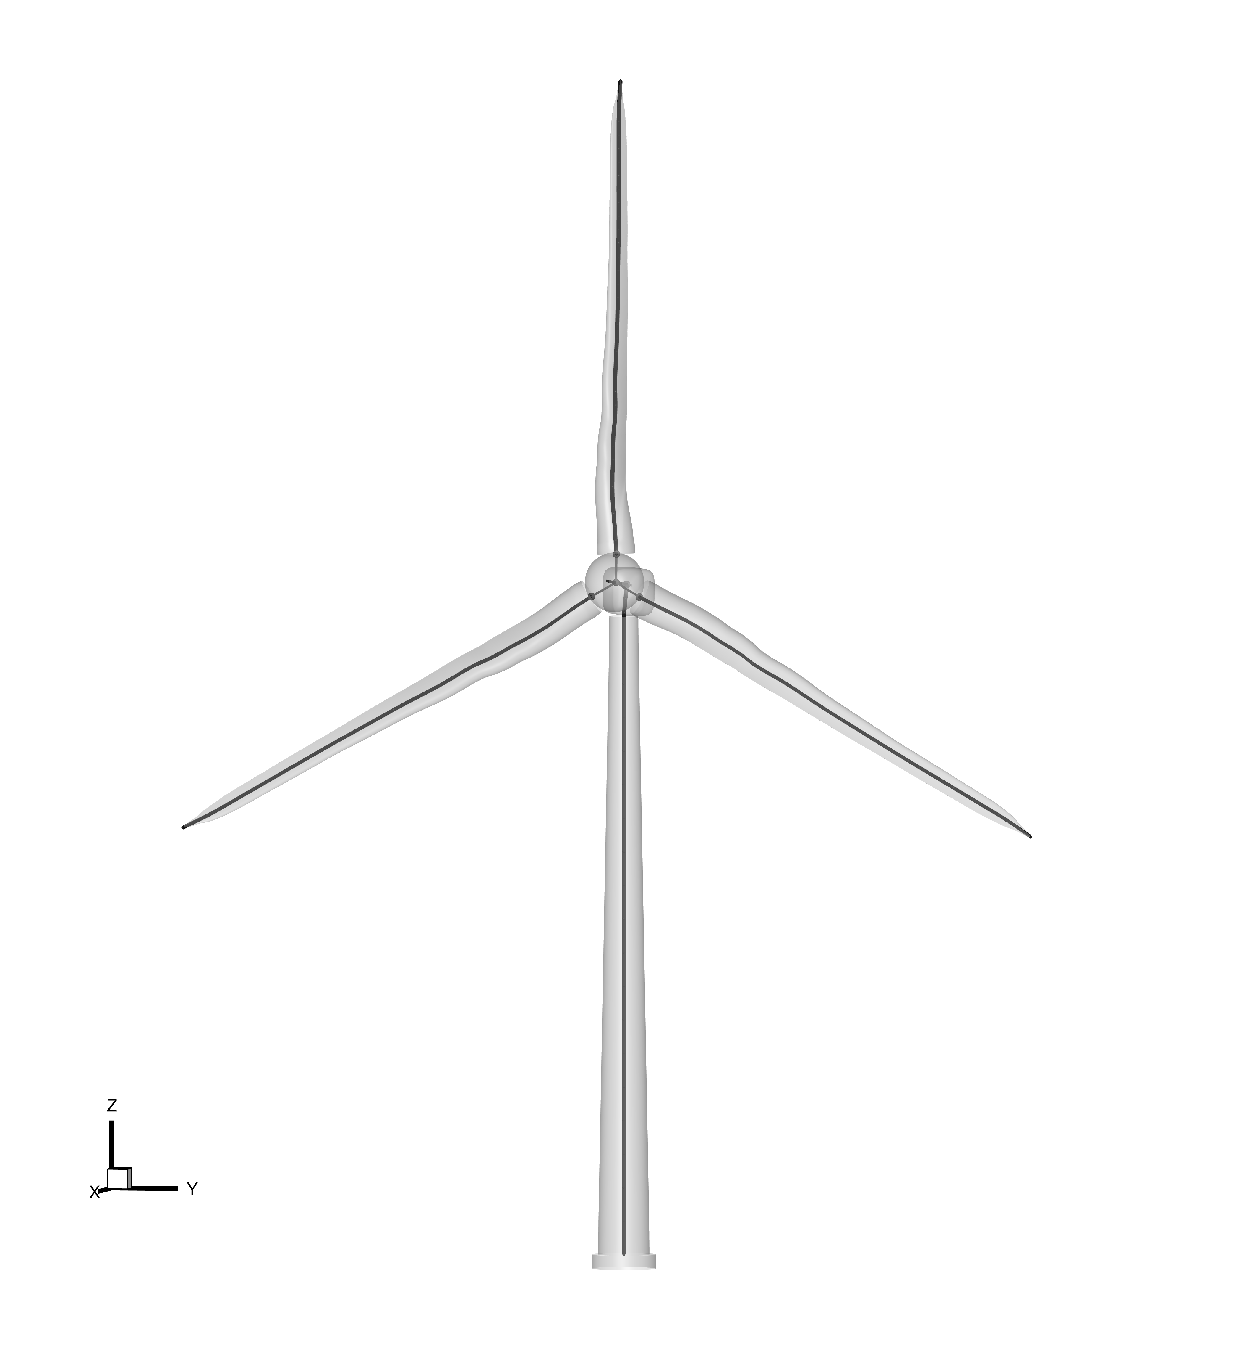
\includegraphics[trim={36.855bp 32.226bp 94.327bp 32.084bp},clip,width=.92\columnwidth,height=.31\textheight,keepaspectratio]{figures/tecplot/turbina_3d.pdf}
\caption{Wind turbine structural idealization: flexible tower and blades, rigid nacelle and hub. Interior lines and nodes identify the beam model. Exterior envelopes are illustrative and represent neither a solid mesh nor CAD geometry.}\label{fig:modelo}
\end{figure}

\subsection{Configurations and component convention}
A material body is the set of particles that constitutes a component. Its reference configuration $\mathcal B_0$ assigns a position $\bm X$ to each particle; its current configuration $\mathcal B_t$ contains the positions occupied at time $t$. Motion is expressed as

\begin{equation}
\bm x=\bm\chi(\bm X,t),\qquad
\bm U(\bm X,t)=\bm\chi(\bm X,t)-\bm X.
\label{eq:configuraciones}
\end{equation}

The reference is the assembly geometry without elastic deformation of the components. The field $\bm U$ contains both rigid motion and deformation: rotor rotation can produce a large displacement without deforming the blades. The symbol $\bm u$ is therefore reserved for structural displacement relative to nominal motion, rather than total displacement $\bm U$.

Vectors and tensors are written in bold; in matrix products, their components in the indicated basis are understood. The symbol $\tr$ denotes transposition, $\I$ is the three-dimensional identity, and $\bm a\otimes\bm b$ is the tensor product, whose matrix is $\bm a\bm b^\tr$. The skew-symmetric matrix associated with the cross product is defined by

\begin{equation}
\Sx{a}=
\begin{bmatrix}0&-a_3&a_2\\a_3&0&-a_1\\-a_2&a_1&0\end{bmatrix},
\qquad \Sx{a}\bm b=\bm a\times\bm b.
\label{eq:skew}
\end{equation}

A rotation matrix transforms components without changing the physical vector. The convention is

\begin{equation}
\bm a^A=\bm Q_{AB}\bm a^B,\qquad
\bm Q_{AC}=\bm Q_{AB}\bm Q_{BC},\qquad
\bm Q_{BA}=\bm Q_{AB}^\tr,
\label{eq:cambio-base}
\end{equation}

where the columns of $\bm Q_{AB}$ are the axes of basis $B$ expressed in $A$. These matrices satisfy $\bm Q^\tr\bm Q=\I$ and $\det\bm Q=1$. A second-order tensor transforms as $\bm J^A=\bm Q_{AB}\bm J^B\bm Q_{AB}^\tr$. Tensor and vector transformations therefore involve different operations.
Figure~\ref{fig:cambio-componentes} illustrates the distinction: the physical vector is unique, whereas its projections depend on the basis. The drawings use $\bm e_i^A$ for axis $i$ of frame $A$; its components in $N$ form column $i$ of $\bm Q_{NA}$.

\begin{figure*}[tp]
\centering
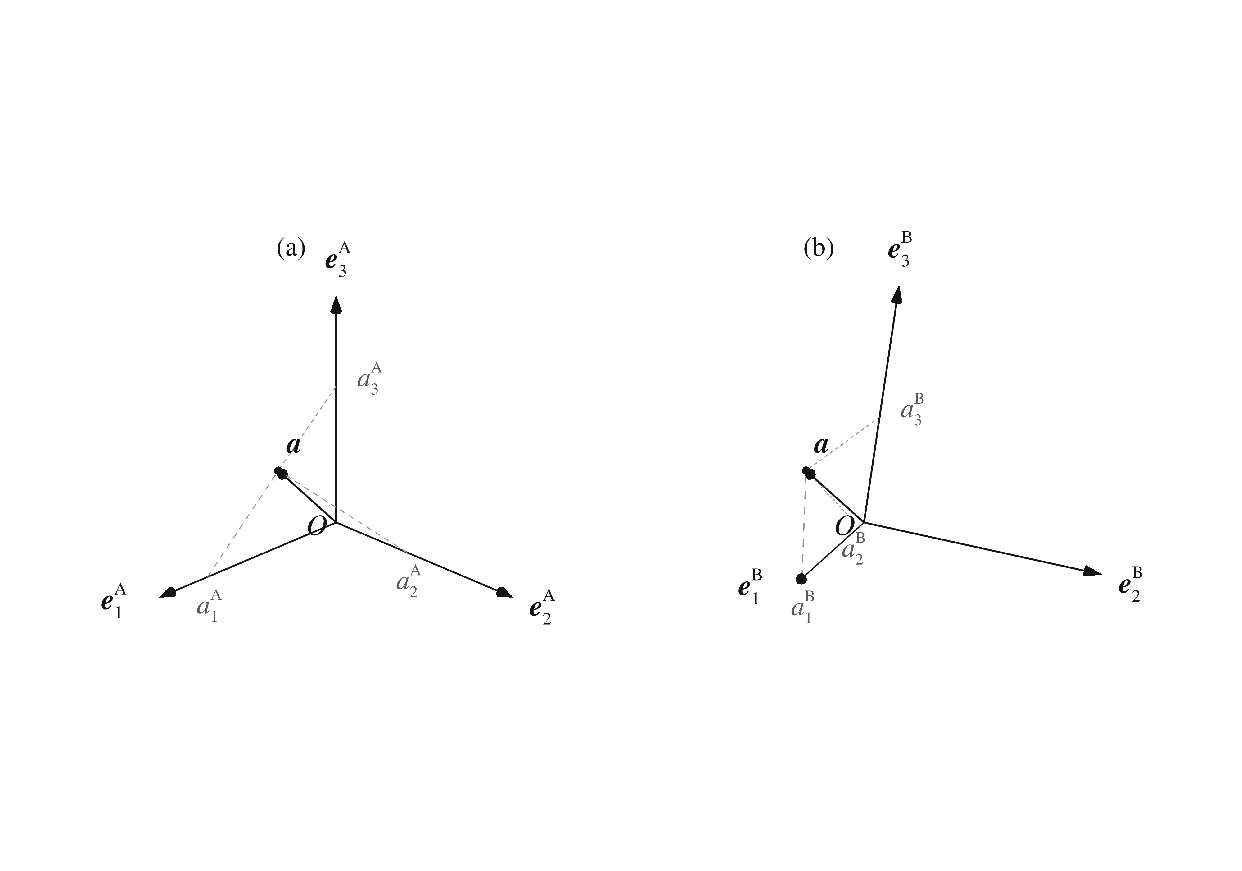
\includegraphics[trim={42.574bp 112.234bp 41.680bp 104.770bp},clip,width=.90\textwidth,height=.30\textheight,keepaspectratio]{figures/tecplot/concept_cambio-componentes.pdf}
\caption{The same vector $\bm a$ expressed in bases (a) $A$ and (b) $B$. Auxiliary lines show its projections. Transformation $\bm a^A=\bm Q_{AB}\bm a^B$ changes components while preserving the geometric vector.}\label{fig:cambio-componentes}
\end{figure*}

\subsection{Reference frames and nominal rotation}
The Newtonian frame $\mathcal F_N=\{O_N;\bm E_1,\bm E_2,\bm E_3\}$ is treated as inertial. The vector $\bm E_3$ is vertical, $\bm E_1$ points along the mean wind, and $\bm E_2=\bm E_3\times\bm E_1$. The base frame $\mathcal F_B$ has axes parallel to those of $N$ and origin $\bm c_B(t)=\bm c_{B0}+\bm u_g(t)$; $\bm u_g$ is the prescribed ground translation. Thus, $\bm Q_{NB}=\I$, but $B$ is not inertial when $\ddot{\bm u}_g\ne\bm0$.

Frame $\mathcal F_G$ originates at the nacelle reference point. Its nominal orientation coincides with that of $N$. Frame $\mathcal F_H$ originates on the hub axis and rotates nominally relative to $G$. An overbar distinguishes nominal from perturbed orientations. Thus,

\begin{align}
\overline{\bm Q}_{NG}&=\I,\qquad
\overline{\bm Q}_{NH}(t)=\bm R_1(\psi(t)),\nonumber\\
\bm R_1(\psi)&=
\begin{bmatrix}1&0&0\\0&\cos\psi&-\sin\psi\\0&\sin\psi&\cos\psi\end{bmatrix},\nonumber\\
\psi(t)&=\psi_0+\Omega t,\qquad \Omega=\text{constant}.
\label{eq:rotacion-nominal}
\end{align}

The azimuth $\psi$ follows the right-hand rule about $\bm E_1$; $\psi_0$ is its initial value, and $\Omega$ is measured in radians per second. Nominal nacelle yaw to follow changes in wind direction is excluded. Small nacelle, hub, and tower vibrations are included in the structural response.
Figure~\ref{fig:sistemas-globales} locates the origins and the three directions of each frame in space. Figure~\ref{fig:giro-nominal} shows the rotation of the hub axes relative to the inertial axes. The superscript $H,n$ in the drawings denotes the nominal orientation represented by an overbar in the text.

\begin{figure*}[tp]
\centering
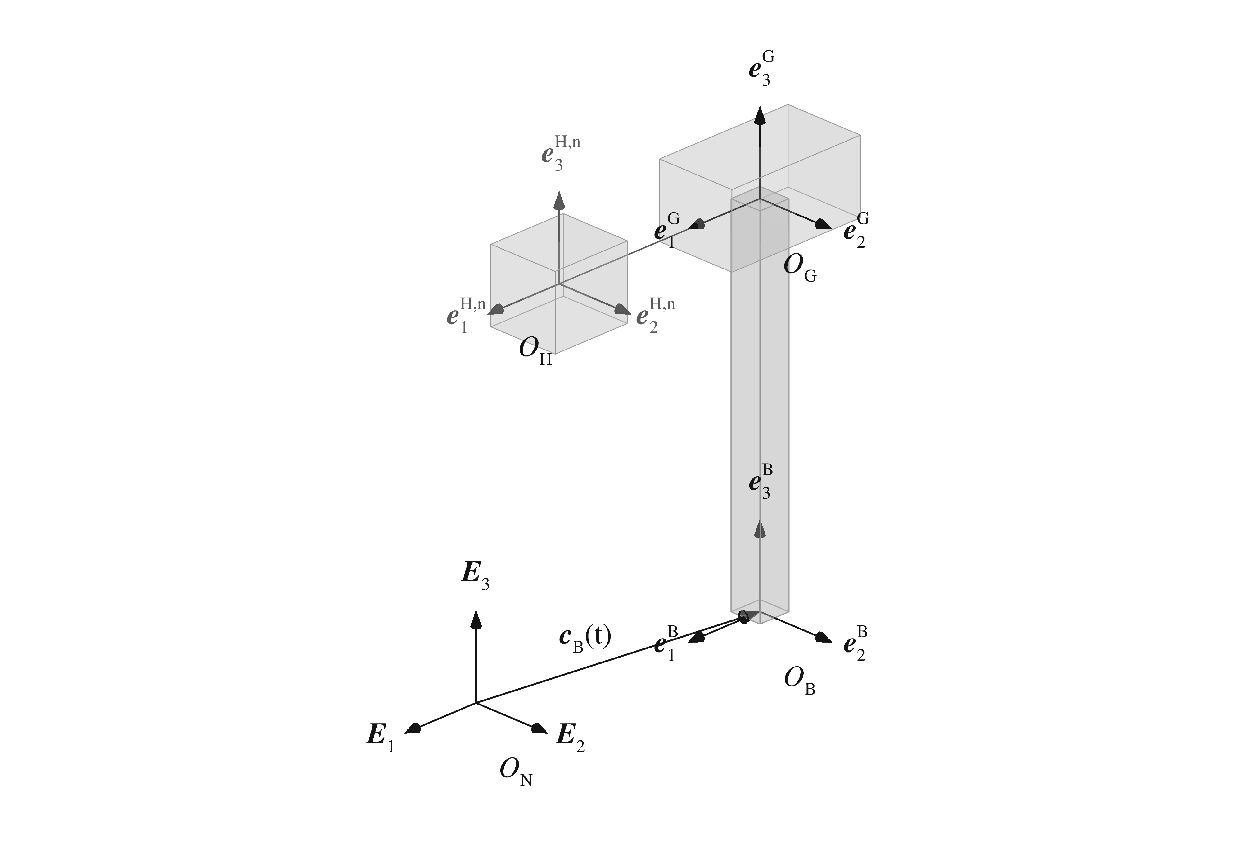
\includegraphics[trim={169.820bp 26.585bp 172.651bp 18.065bp},clip,width=.83\textwidth,height=.35\textheight,keepaspectratio]{figures/tecplot/concept_sistemas-lateral.pdf}
\caption{Reference origins and triads in a spatial view at zero nominal azimuth. The axes of $B$ and $G$ are parallel to the inertial axes; $\bm c_B(t)$ locates the base. Superscript $H,n$ identifies the nominal hub triad. Separations and volumes are schematic.}\label{fig:sistemas-globales}
\end{figure*}

\begin{figure*}[tp]
\centering
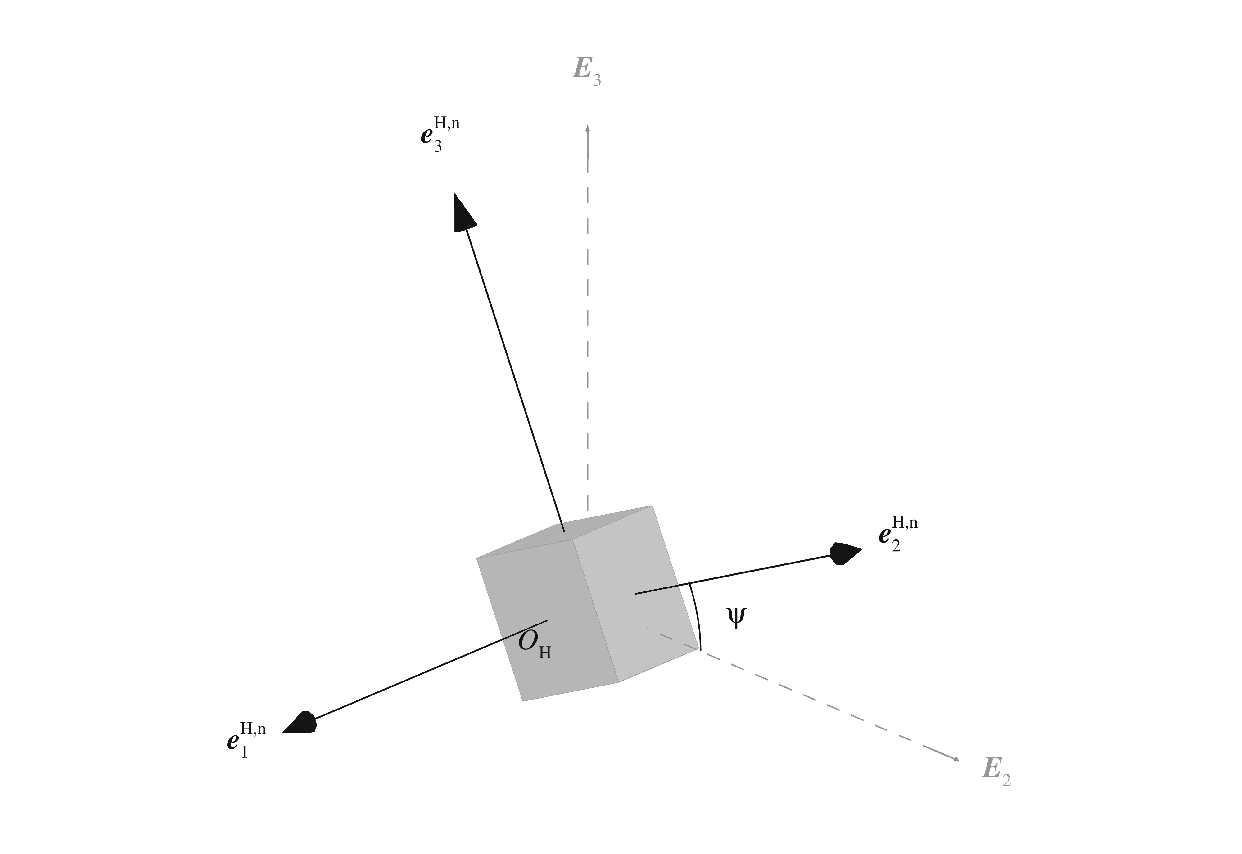
\includegraphics[trim={103.068bp 26.585bp 104.707bp 21.353bp},clip,width=.70\textwidth,height=.29\textheight,keepaspectratio]{figures/tecplot/concept_cubo-nominal.pdf}
\caption{Nominal hub rotation about the common axis 1. Inertial axes 2 and 3 are dashed; nominal axes $H,n$ are solid. Arc $\psi$ follows the right-hand rule. Nominal orientation may be large independently of small structural rotations.}\label{fig:giro-nominal}
\end{figure*}

Each blade $b=1,2,3$ has a root frame $\mathcal F_{P_b}$. Axis 1 is longitudinal, axis 2 is tangential to the rotor, and axis 3 is normal to the rotor plane. For equally spaced blades without initial cone or pitch, define

\begin{align}
\beta_b&=\frac{2\pi(b-1)}3,\qquad
\bm Q_{\rm mont}=
\begin{bmatrix}0&0&1\\0&-1&0\\1&0&0\end{bmatrix},\nonumber\\
\bm Q_{HP_b}&=\bm R_1(\beta_b)\bm Q_{\rm mont},\nonumber\\
\overline{\bm Q}_{NP_b}(t)
&=\overline{\bm Q}_{NH}(t)\bm Q_{HP_b}.
\label{eq:marcos-palas}
\end{align}

The first column of $\bm Q_{HP_b}$ is the radial direction $\bm d_{1b}^H=[0,-\sin\beta_b,\cos\beta_b]^\tr$. The second is $\bm d_{2b}^H=[0,-\cos\beta_b,-\sin\beta_b]^\tr$, and the third is $\bm d_{3b}^H=[1,0,0]^\tr$. Blade 1 points upward when $\psi=0$. If $r_h$ is the distance from the hub origin to the root, its nominal position is

\begin{equation}
\overline{\bm c}_{P_b}^N
=\overline{\bm c}_H^N+\overline{\bm Q}_{NH}\bm r_{b0},
\qquad \bm r_{b0}=r_h\bm d_{1b}^H.
\label{eq:raices}
\end{equation}

A fixed pitch angle $\alpha_b$ is introduced by right-multiplying $\bm Q_{HP_b}$ by $\bm R_1(\alpha_b)$, since it is a rotation about the blade longitudinal axis. This assembly orientation is distinct from azimuth and elastic twist.
Figure~\ref{fig:marcos} specializes the three root bases to zero azimuth. The first index of $\bm d_{ib}$ identifies the axis and the second identifies the blade.

\begin{figure*}[tp]
\centering
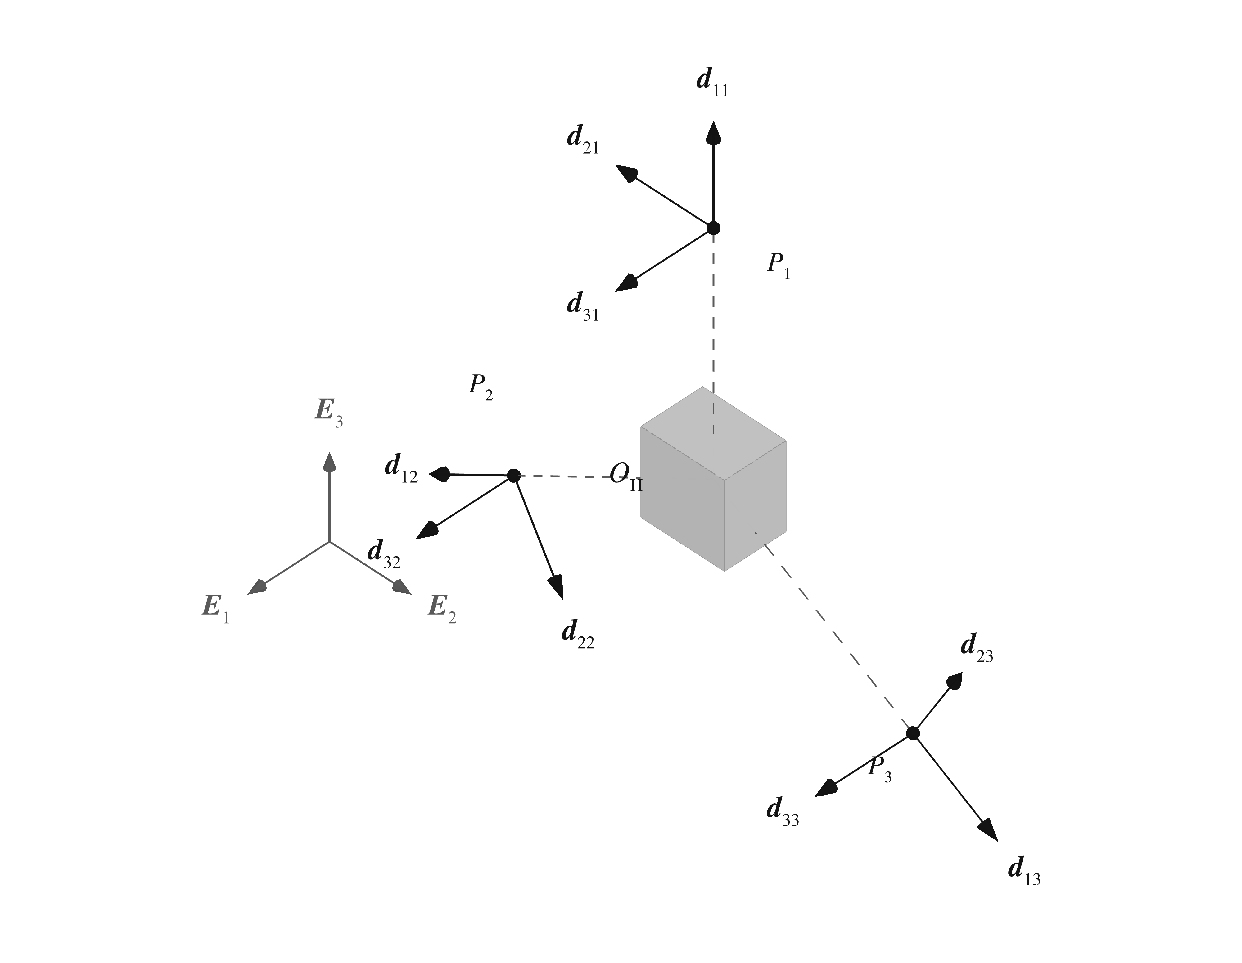
\includegraphics[trim={90.701bp 31.277bp 90.701bp 25.738bp},clip,width=.83\textwidth,height=.37\textheight,keepaspectratio]{figures/tecplot/concept_marcos.pdf}
\caption{The three root triads at $\psi=0$. Director $\bm d_{1b}$ is longitudinal, $\bm d_{2b}$ is tangential, and $\bm d_{3b}=\bm E_1$ completes the right-handed basis. Roots $P_b$ are separated by $120^\circ$ about $O_H$.}\label{fig:marcos}
\end{figure*}

The rotation in Eq.~\eqref{eq:rotacion-nominal} is prescribed: it is supplied to the model rather than calculated from a drive balance. Nominal rotation is prescribed while small relative connection twist remains an unknown. Prescribing the exact instantaneous hub speed would also require constraining that coordinate. The tower and nacelle do not rotate nominally with the rotor; their displacements arise from base excitation and structural deformation.

\subsection{Continuum kinematics of the components}
The position of a rigid-body particle is written as

\begin{equation}
\bm x(\bm\rho,t)=\bm c(t)+\bm Q(t)\bm\rho,
\label{eq:cuerpo-rigido}
\end{equation}

where $\bm c$ is the position of its reference point and $\bm\rho$ is the constant material vector from that point. Matrix $\bm Q$ transforms components from the body-fixed basis to the inertial basis. For a deformable beam, the cross-section origin and orientation also depend on the longitudinal material coordinate $S$:

\begin{align}
\bm X(S,\xi_2,\xi_3)
&=\bm R(S)+\xi_2\bm D_2(S)+\xi_3\bm D_3(S),\nonumber\\
\bm x(S,\xi_2,\xi_3,t)
&=\bm r(S,t)+\xi_2\bm d_2(S,t)+\xi_3\bm d_3(S,t).
\label{eq:viga-continua}
\end{align}

Here, $\bm R$ and $\bm r$ are the reference and current lines; $\xi_2,\xi_3$ locate the same particle within the section in both configurations. The directors $\bm D_i$ and $\bm d_i$ form orthonormal reference and current bases, respectively. Cross-sections remain planar and rigid in their own plane, but their normal $\bm d_1=\bm d_2\times\bm d_3$ need not coincide with the tangent to $\bm r$. This independence represents shear deformation in Timoshenko theory. No additional warping field is resolved; its torsional effect is included through an equivalent stiffness.

Figure~\ref{fig:viga} locates a beam particle using the reference line and the section directors. Figure~\ref{fig:cortante} distinguishes the section normal from the tangent, making their kinematic independence explicit.

\begin{figure*}[tp]
\centering
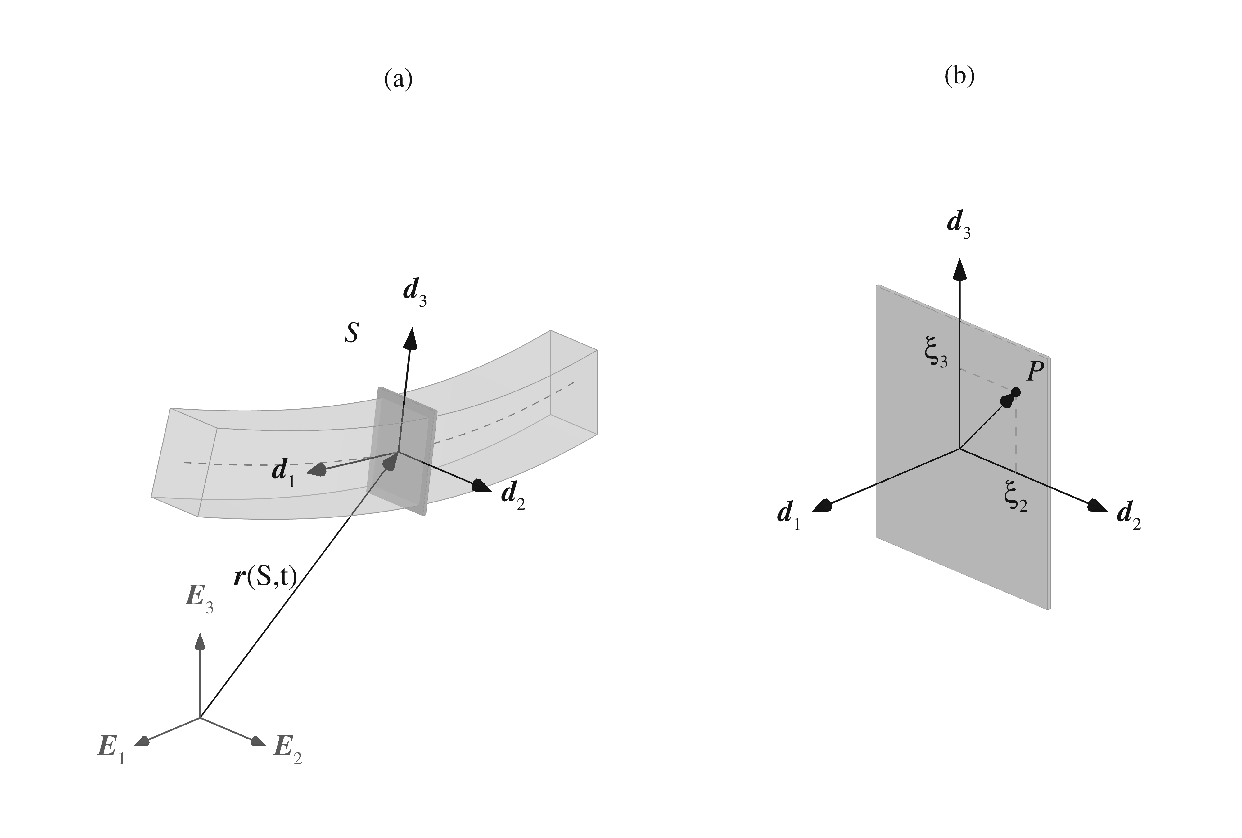
\includegraphics[trim={40.488bp 29.471bp 42.276bp 24.831bp},clip,width=.96\textwidth,height=.34\textheight,keepaspectratio]{figures/tecplot/concept_particula-seccion.pdf}
\caption{Beam-particle position: (a) line $\bm r(S,t)$ and section orientation; (b) sectional detail, where $\bm x_P=\bm r+\xi_2\bm d_2+\xi_3\bm d_3$. The transparent envelope reveals the reference line; its surfaces add no degrees of freedom.}\label{fig:viga}
\end{figure*}

\begin{figure*}[tp]
\centering
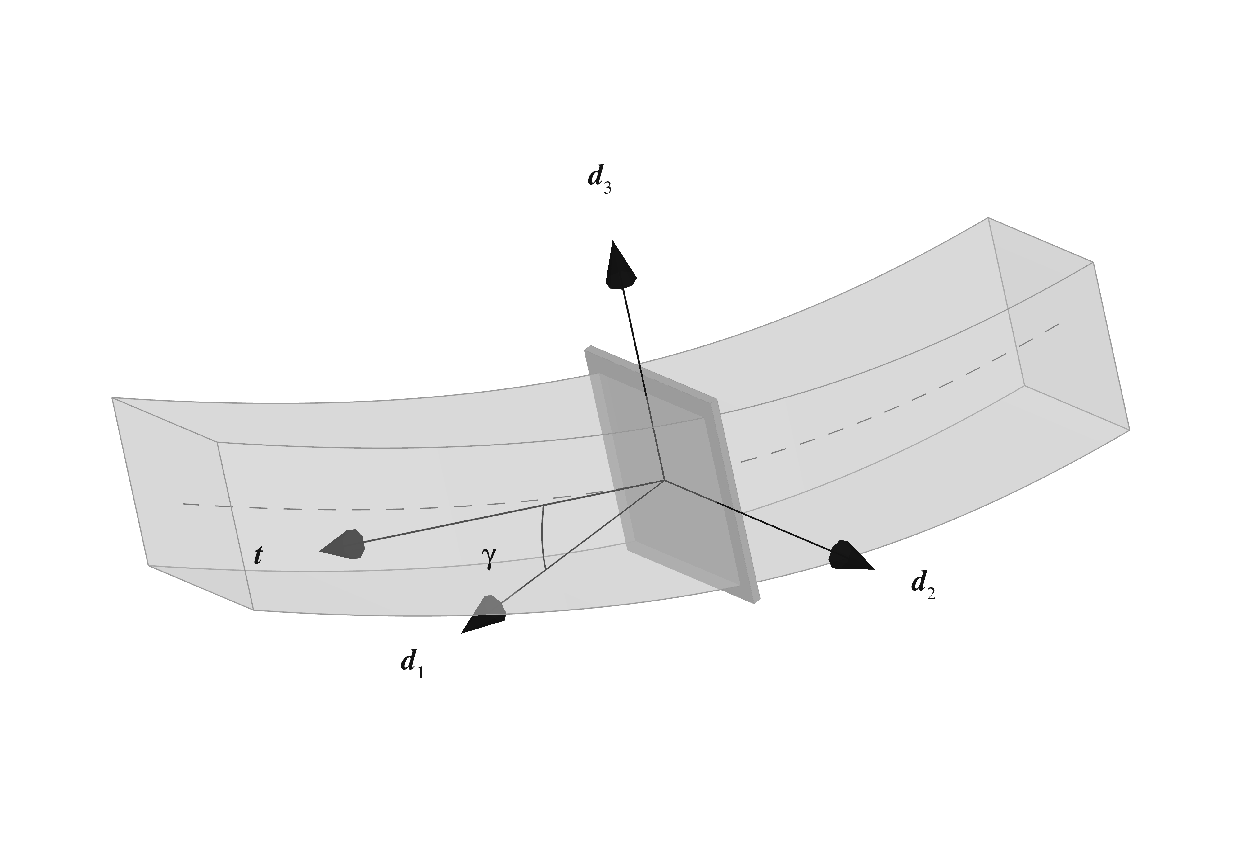
\includegraphics[trim={47.342bp 78.302bp 47.342bp 72.622bp},clip,width=.82\textwidth,height=.32\textheight,keepaspectratio]{figures/tecplot/concept_shear.pdf}
\caption{Independence of section normal $\bm d_1$ and reference-line tangent $\bm t$. Angle $\gamma$ illustrates shear in the drawing plane; it is an illustrative angular component, rather than the complete strain vector $\bm\gamma$ in Eq.~\eqref{eq:medidas-viga}.}\label{fig:cortante}
\end{figure*}

For a straight blade, the nominal line position is obtained by adding $\overline{\bm Q}_{NP_b}[S,0,0]^\tr$ to Eq.~\eqref{eq:raices}. In the tower, $S$ runs from the base to the nacelle, with nominal triad $(\bm E_3,\bm E_1,\bm E_2)$. This defines the relationship between each beam's material coordinates and the machine geometry.

Perturbation rotation is represented by $\bm E(\bm\theta)=\exp(\Sx{\theta})$. For the nacelle and hub, $\bm Q=\overline{\bm Q}\bm E$; the same relation applies to a section after including its assembly orientation. Vector $\bm\theta$ expresses the angular increment in the corresponding nominal basis. It is generally neither a vector of Euler angles nor a quantity whose derivative equals angular velocity exactly. That relationship is specified when the inertial terms are derived.

Figure~\ref{fig:configuraciones} compares the material reference, nominal motion, and perturbed motion. The position a particle would have under nominal motion is denoted by $\overline{\bm x}(\bm X,t)$, and the corresponding configuration by $\overline{\mathcal B}_t$. The difference $\bm x-\overline{\bm x}$ is its displacement relative to that trajectory; in a beam, this includes both translation of the section origin and the change in section orientation.

\begin{figure*}[tp]
\centering
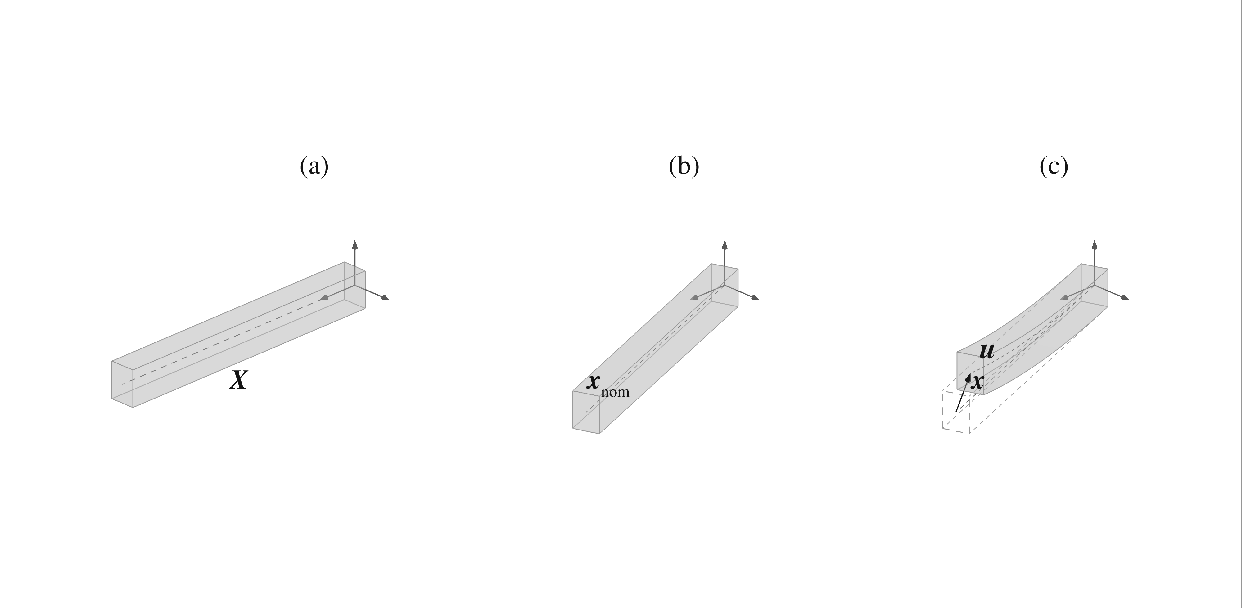
\includegraphics[trim={47.491bp 0.000bp 0.000bp 0.000bp},clip,width=.98\textwidth,height=.24\textheight,keepaspectratio]{figures/tecplot/concept_tresniveles.pdf}
\caption{The same material portion in (a) reference, (b) nominal motion, and (c) perturbed configuration. In (c), the dashed contour repeats the nominal configuration, and arrow $\bm u$ indicates the endpoint difference. Here, $\bm x_{\rm nom}$ denotes $\overline{\bm x}$; displacements are enlarged to distinguish the states.}\label{fig:configuraciones}
\end{figure*}

Deformation is measured relative to the material geometry, independently of the observer. For example, if $\bm Q_s=[\bm d_1,\bm d_2,\bm d_3]$ and $\bm Q_{s0}=[\bm D_1,\bm D_2,\bm D_3]$, the extension--shear and curvature--twist measures are

\begin{align}
\bm\gamma&=\bm Q_s^\tr\bm r'-\bm Q_{s0}^\tr\bm R',\nonumber\\
\bm\kappa&=\operatorname{axial}(\bm Q_s^\tr\bm Q_s')
-\operatorname{axial}(\bm Q_{s0}^\tr\bm Q_{s0}').
\label{eq:medidas-viga}
\end{align}

A prime denotes differentiation with respect to $S$, and $\operatorname{axial}([\bm a]_\times)=\bm a$. A superposed rigid motion leaves these measures unchanged. For an initially straight beam, their linear approximation in structural translations and rotations is used; nominal rotation is retained separately.

\subsection{Operating state and perturbations}
The material geometry $\mathcal B_0$, prescribed nominal trajectory, and structural equilibrium configuration $\bm q_0$ are distinguished. The latter depends on loads, rotational speed, and component properties. Structural coordinates are written as $\bm q(t)=\bm q_0+\delta\bm q(t)$; $\delta\bm q$ describes vibrations without including the prescribed azimuth again.

When loads and coefficients are stationary in the chosen coordinates, $\bm q_0$ defines relative equilibrium: deformation is constant in those coordinates although rotor particles continue moving. Gravity fixed in the inertial frame or nonuniform flow may prevent this stationarity. In that case, equilibrium at a given azimuth and its linearization are a local approximation, rather than a complete periodic solution. Reference mass properties are retained; preload modifies the tangent stiffness within the small-deformation assumption.

\FloatBarrier
\section{Section properties and mass}
\subsection{Geometric and mass moments of inertia}
Properties are defined on a material section $A_0(S)$ using reference density $\rho_0$ and local coordinates $y,z$. The geometric second-moment tensor about the geometric center is

\begin{equation}
\bm I_A=\int_{A_0}
\big[(\bm\xi\cdot\bm\xi)\I-\bm\xi\otimes\bm\xi\big]\,\dd A,
\qquad \bm\xi=[0,y,z]^\tr.
\end{equation}

This gives $I_y=\int_{A_0}z^2\dd A$, $I_z=\int_{A_0}y^2\dd A$, and the polar moment $I_y+I_z$. The area is $A=\int_{A_0}\dd A$. In principal axes and for a section without constitutive coupling, the sectional stiffness matrix is

\begin{equation}
\bm K_s=\operatorname{diag}(EA,GA_{sy},GA_{sz},GJ_t,EI_y,EI_z),
\label{eq:Ks}
\end{equation}

where $E$ is Young's modulus, $G$ is the shear modulus, $A_{sy},A_{sz}$ are effective shear areas, and $J_t$ is the torsional constant. The effective areas already include the correction for the shear-stress distribution. The quantities $I_y,I_z,J_t$ have units of $\mathrm{m^4}$, but $J_t$ does not generally equal $I_y+I_z$. The matrix relates generalized strains to their work-conjugate resultants:

\begin{equation}
\begin{bmatrix}\bm n\\\bm m_s\end{bmatrix}
=\bm K_s\begin{bmatrix}\bm\gamma\\\bm\kappa\end{bmatrix}.
\label{eq:constitutiva}
\end{equation}

The components of $\bm n$ are the axial and two shear forces; those of $\bm m_s$ are the torsional and two bending moments. They follow by integrating sectional traction $\bm t$ and its moment: $\bm n=\int_{A_0}\bm t\,\dd A$ and $\bm m_s=\int_{A_0}\bm\xi\times\bm t\,\dd A$, within the small-deformation approximation. Their work per unit length is $\bm n\cdot\delta\bm\gamma+\bm m_s\cdot\delta\bm\kappa$. A composite or eccentric section may require a full symmetric constitutive matrix; the diagonal expression~\eqref{eq:Ks} assumes those couplings are negligible.

Mass properties use the sectional center of mass $C$, which need not coincide with the geometric center. If $\bm\rho_C$ connects $C$ to a sectional particle,

\begin{align}
\mu&=\int_{A_0}\rho_0\,\dd A,\qquad
\int_{A_0}\rho_0\bm\rho_C\,\dd A=\bm0,\nonumber\\
\bm j_C&=\int_{A_0}\rho_0
\big[(\bm\rho_C\cdot\bm\rho_C)\I-\bm\rho_C\otimes\bm\rho_C\big]\,\dd A.
\label{eq:sectioninertia}
\end{align}

In centroidal principal axes, $j_y=\int_{A_0}\rho_0 z^2\dd A$, $j_z=\int_{A_0}\rho_0 y^2\dd A$, and $j_x=j_y+j_z$ for a planar section. The units of $\mu$ and $\bm j_C$ are $\mathrm{kg/m}$ and $\mathrm{kg\,m}$. Off-diagonal entries are the negatives of the integrated coordinate products. This distinguishes a mass-inertia tensor from a geometric second moment of area.

For a homogeneous isotropic material, $G=E/[2(1+\nu)]$, where $\nu$ is Poisson's ratio; also, $\mu=\rho_0 A$ and $\bm j_C=\rho_0\operatorname{diag}(I_y+I_z,I_y,I_z)$. Blade stiffnesses and mass properties may come directly from a sectional analysis. If a tabulated distribution must be normalized to a known total mass $m_b^\star$ while preserving its spatial shape and radii of gyration, use

\begin{equation}
c_b=\frac{m_b^\star}{\int_0^{L_b}\mu^{\rm tab}(S)\,\dd S},
\qquad (\mu,\bm j_C)=c_b(\mu^{\rm tab},\bm j_C^{\rm tab}).
\label{eq:massscale}
\end{equation}

Here, $L_b$ is blade length, and superscript $\mathrm{tab}$ identifies the input data. Factor $c_b$ is dimensionless and applies to the full tensor. This normalization does not determine eccentricities or inertia products absent from the data. Assuming them to be zero is an additional idealization that must be consistent with the adopted section axes.

\subsection{Spatial mass matrix}
Let $\bm r_C$ be the vector from the section origin to its center of mass, expressed in the same basis as the velocities. The centroidal velocity is $\bm v_C=\bm v_O+\bm\omega_s\times\bm r_C$, where $\bm v_O$ and $\bm\omega_s$ are the origin velocity and section angular velocity. Integrating particle energy and using the centroidal condition eliminates the cross term about $C$, giving

\begin{equation}
\mathcal T_s=\tfrac12\mu\|\bm v_C\|^2
+\tfrac12\bm\omega_s^\tr\bm j_C\bm\omega_s.
\label{eq:energia-seccion}
\end{equation}

Figure~\ref{fig:masa-seccional} distinguishes the reference-line origin, center of mass, and particle position. Vector $\bm r_C+\bm\rho_C$ locates the particle from the origin; tensor $\bm j_C$ in Eq.~\eqref{eq:sectioninertia} instead uses distances measured from $C$.

\begin{figure*}[tp]
\centering
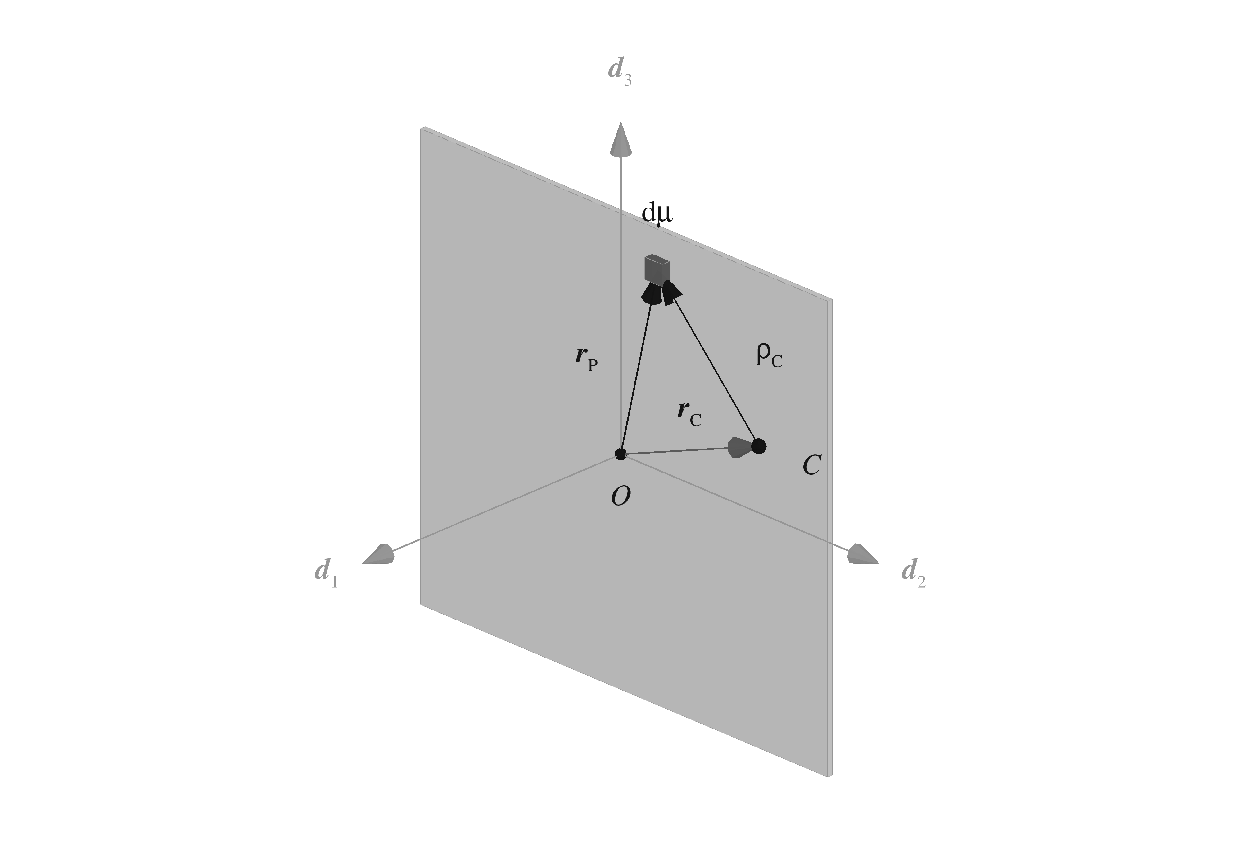
\includegraphics[trim={145.086bp 30.620bp 145.682bp 21.054bp},clip,width=.76\textwidth,height=.30\textheight,keepaspectratio]{figures/tecplot/paper_masa_seccional.pdf}
\caption{Mass-integration geometry: section origin $O$, center of mass $C$, and contribution $\dd\mu=\rho_0\dd A$. Particle position satisfies $\bm r_P=\bm r_C+\bm\rho_C$. Centroidal inertia uses $\bm\rho_C$; transfer to the origin uses $\bm r_C$. Section thickness is illustrative.}\label{fig:masa-seccional}
\end{figure*}

To express this energy relative to the section origin, introduce

\begin{equation}
\bm B_C=[\I,-\Sx{r_C}],\qquad \bm E_\theta=[\bm0,\I].
\end{equation}

In a stationary reference and at first kinematic order, $[\bm v_O^\tr,\bm\omega_s^\tr]^\tr=\dot{\bm\eta}$, with $\bm\eta=[\bm u^\tr,\bm\theta^\tr]^\tr$. The quadratic energy is then

\begin{equation}
\mathcal T_s=\tfrac12\mu\|\bm B_C\dot{\bm\eta}\|^2
+\tfrac12(\bm E_\theta\dot{\bm\eta})^\tr\bm j_C(\bm E_\theta\dot{\bm\eta}),
\end{equation}

The matrix multiplying these generalized velocities is therefore

\begin{equation}
\bm M_s=\begin{bmatrix}
\mu\I&-\mu\Sx{r_C}\\
\mu\Sx{r_C}&\bm j_C-\mu\Sx{r_C}^2
\end{bmatrix}.
\label{eq:Ms}
\end{equation}

The block $-\mu\Sx{r_C}^2=\mu[(\bm r_C\cdot\bm r_C)\I-\bm r_C\otimes\bm r_C]$ follows from the parallel-axis theorem. Cross blocks represent translation--rotation coupling due to eccentricity. During nominal rotation, the energy contains additional terms, which are derived rather than identifying total angular velocity with $\dot{\bm\theta}$.

For a rigid body, replace $\mu$ by $m=\int_{\mathcal B_0}\rho_0\,\dd V$ and $\bm j_C$ by $\bm J_C=\int_{\mathcal B_0}\rho_0[(\bm\rho_C\cdot\bm\rho_C)\I-\bm\rho_C\otimes\bm\rho_C]\,\dd V$, with units of $\mathrm{kg\,m^2}$. Transformation~\eqref{eq:cambio-base} expresses the tensor in the assembly basis, and the parallel-axis theorem refers it to the chosen nacelle or hub point. Orientation and eccentricity act on the full tensor, rather than only its diagonal entries.

\section{Structural discretization}
\label{sec:elementos}
\subsection{Nodal variables and interpolation}
Each beam reference line is divided into two-node elements. Each node has three structural translations and three rotations, so $\bm q_i=[\bm u_i^\tr,\bm\theta_i^\tr]^\tr$ and each element has twelve coordinates before constraints. Local coordinate $x\in[0,L]$ spans the element reference length, corresponding to an interval of material coordinate $S$. Local axes $x,y,z$ coincide with section axes 1, 2, and 3. In these axes, linearizing Eq.~\eqref{eq:medidas-viga} for the field $\bm\eta=[u,v,w,\theta_x,\theta_y,\theta_z]^\tr$ gives

\begin{equation}
\bm\varepsilon=[u',v'-\theta_z,w'+\theta_y,
\theta_x',\theta_y',\theta_z']^\tr.
\end{equation}

The first three components are extension and shear; the last three are twist and curvatures. A prime now denotes differentiation with respect to $x$. Interpolation is $\bm\eta=\bm N(x)\bm q_e^\ell$, where $\bm N$ has size $6\times12$ and $\ell$ identifies local components. Substitution into the strain relations gives $\bm\varepsilon=\bm B(x)\bm q_e^\ell$. Internal virtual work and kinetic energy yield the element matrices

\begin{align}
U_e&=\tfrac12\int_0^L\bm\varepsilon^\tr\bm K_s\bm\varepsilon\,\dd x,\nonumber\\
\bm K_e^\ell&=\int_0^L\bm B^\tr\bm K_s\bm B\,\dd x,\nonumber\\
\bm M_e^\ell&=\int_0^L\bm N^\tr\bm M_s\bm N\,\dd x.
\label{eq:elementenergy}
\end{align}

A closed-form two-node interpolation is used for uncoupled properties constant within each element \citep{reddy2006}. Stiffness blocks and the functions used for mass are detailed in Appendix A. The limit $GA_s\to\infty$ removes shear deformation; if rotary inertia is retained, the limiting dynamic model is of Rayleigh type, rather than classical Euler--Bernoulli.

\subsection{Orientation and assembly}
The reference end positions $\bm X_I,\bm X_J$ and an auxiliary point $\bm X_a$ determine the element basis:

\begin{align}
L&=\|\bm X_J-\bm X_I\|,\quad
\bm e_1=(\bm X_J-\bm X_I)/L,\nonumber\\
\bm p&=(\I-\bm e_1\bm e_1^\tr)(\bm X_a-\bm X_I),\nonumber\\
\bm e_3&=\bm p/\|\bm p\|,\qquad
\bm e_2=\bm e_3\times\bm e_1.
\label{eq:base-elemento}
\end{align}

The auxiliary point must lie off the axis and is chosen to reproduce the sectional assembly directions. With $\bm Q_e=[\bm e_1,\bm e_2,\bm e_3]$ and $\bm R_e=\bm Q_e^\tr$,

\begin{equation}
\bm q_e^\ell=\bm T_e\bm q_e^g,\qquad
\bm T_e=\operatorname{diag}(\bm R_e,\bm R_e,\bm R_e,\bm R_e).
\end{equation}

Superscript $g$ identifies assembly components, whose axes are parallel to those of $N$ for the geometry considered. The symbol $\operatorname{diag}$ with matrix arguments denotes a block-diagonal matrix. Conservation of virtual work gives $\bm K_e^g=\bm T_e^\tr\bm K_e^\ell\bm T_e$ and $\bm M_e^g=\bm T_e^\tr\bm M_e^\ell\bm T_e$. This transformation at a given configuration does not replace the time-dependent transformation of velocities and accelerations.

Figure~\ref{fig:elemento} identifies the element ends and the projected auxiliary direction used to construct its spatial basis. The auxiliary point fixes only the transverse axes; it is not a node with degrees of freedom.

\begin{figure*}[tp]
\centering
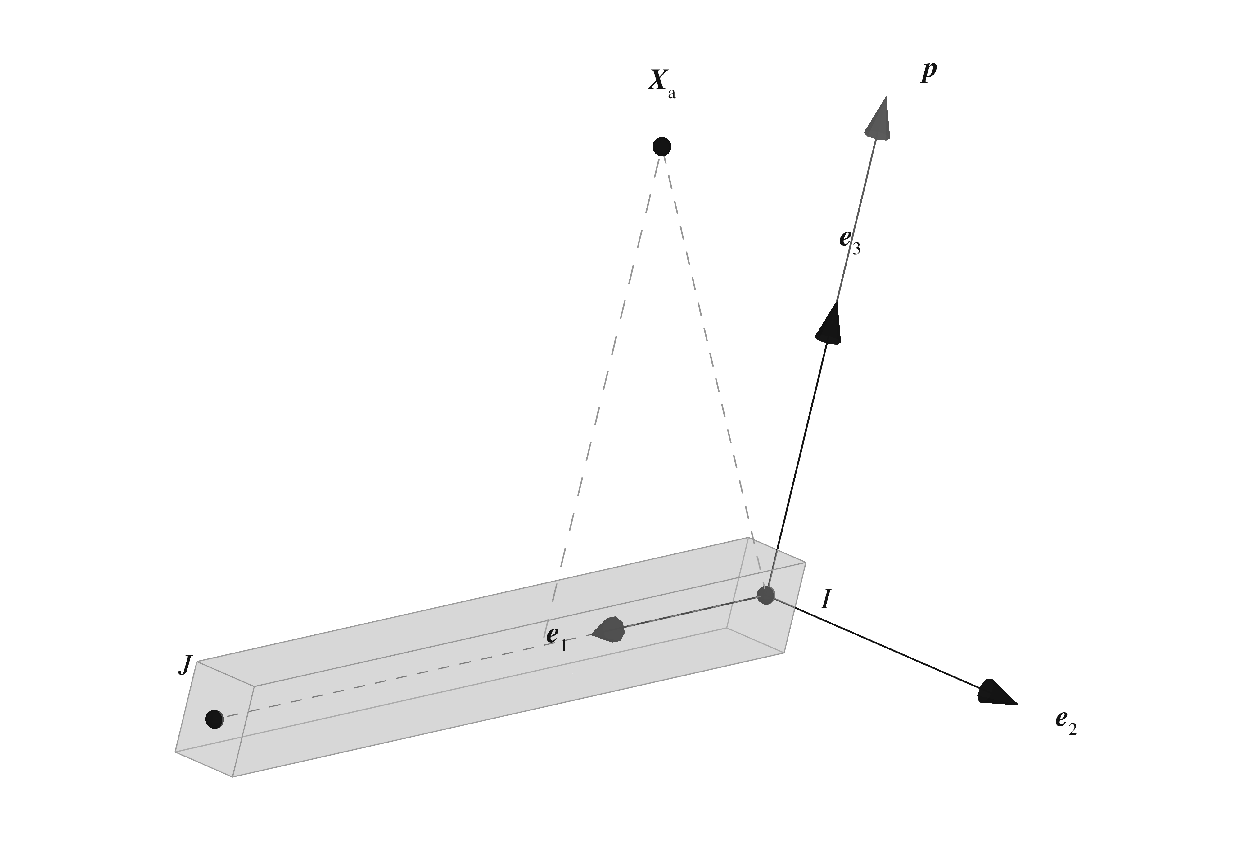
\includegraphics[trim={77.738bp 30.620bp 72.970bp 24.343bp},clip,width=.82\textwidth,height=.32\textheight,keepaspectratio]{figures/tecplot/concept_elemento.pdf}
\caption{Orientation of an element between $I$ and $J$. Axis $\bm e_1$ follows the chord; projection $\bm p$ of auxiliary point $\bm X_a$ onto the normal plane determines $\bm e_3$. The triad is completed by $\bm e_2=\bm e_3\times\bm e_1$. The auxiliary point is not a structural node.}\label{fig:elemento}
\end{figure*}

If $\bm L_e$ extracts the element coordinates from $\bm q$, a generic matrix $\bm A$, such as mass or stiffness, is assembled as

\begin{equation}
\bm A=\sum_e\bm L_e^\tr\bm A_e^g\bm L_e
+\sum_R\bm L_R^\tr\bm A_R^g\bm L_R,
\end{equation}

where $\bm L_R$ locates rigid-body and connection contributions in global coordinates. Kinematic constraints are imposed after assembly, so coordinates on both sides of each connection are still retained.

\subsection{Nacelle--hub connection}
The nacelle and hub reference points $G,H$ are nominally separated by $\bm d=\overline{\bm c}_H-\overline{\bm c}_G$. In a common basis, the relative connection deformation is

\begin{equation}
\bm\Delta_d=\begin{bmatrix}
\bm u_H-\bm u_G+\Sx{d}\bm\theta_G\\
\bm\theta_H-\bm\theta_G
\end{bmatrix}=\bm B_d\bm q.
\end{equation}

Matrix $\bm B_d$ collects the coefficients of this relation; its columns corresponding to $[\bm u_G,\bm\theta_G,\bm u_H,\bm\theta_H]$ are $[-\I,\Sx{d},\I,\bm0]$ in the translational block and $[\bm0,-\I,\bm0,\I]$ in the angular block. Constitutive matrices $\bm k_d,\bm c_d$ relate forces and moments to $\bm\Delta_d,\dot{\bm\Delta}_d$. This gives $\bm K_d=\bm B_d^\tr\bm k_d\bm B_d$ and $\bm C_d=\bm B_d^\tr\bm c_d\bm B_d$. The arm removes spurious deformation under common rigid motion. Relative drivetrain twist is an elastic unknown distinct from nominal rotation; with positive torsional stiffness, it is not a zero-frequency mechanism.

\FloatBarrier
\section{Inertial contributions of prescribed rotation}
\label{sec:giro}
\subsection{Position, velocity, and kinetic energy}
The nominal hub orientation is used as the rotating basis, abbreviated as $\bm R_0(t)=\overline{\bm Q}_{NH}(t)$. Components in this basis are termed \emph{corotating} and identified by subscript $c$. Vector $\bm\Omega=[\Omega,0,0]^\tr$ and matrix $\bm W=\Sx{\Omega}$ satisfy $\dot{\bm R}_0=\bm R_0\bm W$. Since nominal rotation is about a fixed axis parallel to $\bm E_1$, $\bm R_0\bm W\bm R_0^\tr=\bm W$ also holds.

For a blade section, $\bm a$ connects the hub origin to the nominal section origin, and $\bm r$ connects the latter to the center of mass. Both are expressed in the corotating basis. For a straight blade,

\begin{align}
\bm a(S)&=\bm r_{b0}+\bm Q_{HP_b}[S,0,0]^\tr,\nonumber\\
\bm r&=\bm Q_{HP_b}\bm r_C,\qquad
\bm J=\bm Q_{HP_b}\bm j_C\bm Q_{HP_b}^\tr.
\label{eq:datos-giro}
\end{align}

In the following expressions, $m=\mu$ and $\bm J$ is sectional inertia per unit length. The same formulas apply to the hub using its total mass and centroidal tensor. The nominal rotational contributions of the tower and nacelle are zero.

Displacement $\bm u$ and rotation $\bm\theta$ are now expressed in the common corotating basis. Perturbation $\bm E=\exp(\Sx{\theta})$ acts on the reference orientation and eccentricity. The center-of-mass position and its tensor are

\begin{equation}
\bm x_C=\overline{\bm c}_H+\bm R_0(\bm a+\bm u+\bm E\bm r),\qquad
\bm J_C^{c}(\bm\theta)=\bm E\bm J\bm E^\tr.
\end{equation}

The nominal origin $\overline{\bm c}_H$ is fixed during this derivation; base translation is introduced later. For $\vartheta=\|\bm\theta\|$, the rotation and the relation between angular velocity and the derivative of $\bm\theta$ are

\begin{align}
\bm E&=\I+\frac{\sin\vartheta}{\vartheta}\Sx{\theta}
+\frac{1-\cos\vartheta}{\vartheta^2}\Sx{\theta}^2,\nonumber\\
\bm J_\ell&=\I+\frac{1-\cos\vartheta}{\vartheta^2}\Sx{\theta}
+\frac{\vartheta-\sin\vartheta}{\vartheta^3}\Sx{\theta}^2.
\label{eq:jacobiano}
\end{align}

The ratios are evaluated by continuity at $\vartheta=0$. Matrix $\bm J_\ell$ is the left Jacobian of the exponential representation: it satisfies $\dot{\bm E}\bm E^\tr=[\bm J_\ell\dot{\bm\theta}]_\times$. Differentiating the preceding position and adding nominal rotation gives

\begin{align}
\bm v_C&=\bm W(\bm a+\bm u+\bm E\bm r)+\dot{\bm u}
+\Sx{J_\ell(\bm\theta)\dot{\bm\theta}}\bm E\bm r,\nonumber\\
\bm\omega&=\bm\Omega+\bm J_\ell(\bm\theta)\dot{\bm\theta}.
\label{eq:exactvelocity}
\end{align}

Here, $\bm v_C$ denotes corotating components of absolute velocity, and $\bm\omega$ those of absolute angular velocity. For a particle with relative position $\bm y$, the same derivation gives

\begin{equation}
\ddot{\bm x}=\bm R_0
\big(\ddot{\bm y}+2\bm W\dot{\bm y}+\bm W^2\bm y\big).
\label{eq:aceleracion-transporte}
\end{equation}

The terms $2\bm W\dot{\bm y}$ and $\bm W^2\bm y$ are the Coriolis and centripetal-acceleration contributions, respectively. Term $\dot{\bm W}\bm y$ vanishes under the assumption $\Omega=\mathrm{constant}$. The section or body kinetic energy is

\begin{equation}
\mathcal T=\tfrac12m\bm v_C^\tr\bm v_C
+\tfrac12\bm\omega^\tr\bm E\bm J\bm E^\tr\bm\omega.
\label{eq:exactT}
\end{equation}

\subsection{Energy decomposition and linearization}
Energy~\eqref{eq:exactT} is not homogeneous of degree two in structural velocities because the body moves even when $\dot{\bm\eta}=\bm0$. Following the classification of \citet[Sections 4.1 and 4.4]{meirovitch1997}, it can be written as

\begin{align}
\mathcal T&=\mathcal T_2+\mathcal T_1+\mathcal T_0,\nonumber\\
\mathcal T_2&=\tfrac12\dot{\bm\eta}^\tr\bm M(\bm\eta)\dot{\bm\eta},\nonumber\\
\mathcal T_1&=\dot{\bm\eta}^\tr\bm p_T(\bm\eta),\qquad
\mathcal T_0=\mathcal T(\bm\eta,\bm0;\Omega).
\label{eq:descomposicion}
\end{align}

The subscripts indicate degree in $\dot{\bm\eta}$, rather than order in displacements. Matrix $\bm M(\bm\eta)$ and vector $\bm p_T(\bm\eta)$ are the coefficients of this decomposition. In particular, $\mathcal T_0$ depends on position and orientation despite being independent of structural velocities.

Linearization requires an additional operation: expanding the Lagrangian about the nominal state and retaining terms of second degree in displacements, rotations, and their velocities. In the reference-inertia model, components of $\bm\eta=[\bm u^\tr,\bm\theta^\tr]^\tr$ are small, and the expansions are

\begin{align}
\bm E&=\I+\Sx{\theta}+\tfrac12\Sx{\theta}^2+\mathcal O(3),\nonumber\\
\bm J_\ell\dot{\bm\theta}&=\dot{\bm\theta}
+\tfrac12\bm\theta\times\dot{\bm\theta}+\mathcal O(3).
\end{align}

The second-degree terms containing perturbation velocities are collected in

\begin{equation}
\mathcal T_v^{(2)}=\tfrac12\dot{\bm\eta}^\tr\bm M_6\dot{\bm\eta}
+\dot{\bm\eta}^\tr\bm A_6\bm\eta.
\label{eq:T2}
\end{equation}

Superscript $(2)$ indicates total expansion order, unlike the subscript in $\mathcal T_2$; subscript $v$ restricts this expression to the terms needed to derive mass and gyroscopy. The nominal balance and complete tangent follow directly from the equations of motion. To express these coefficients, introduce

\begin{align}
\bm B&=[\I,-\Sx{r}],&\bm E_\theta&=[\bm0,\I],\nonumber\\
\bm b&=\bm a+\bm r,&\bm h&=\bm J\bm\Omega,\nonumber\\
\bm v_0&=\bm W\bm b.
\end{align}

Vector $\bm b$ is the nominal center-of-mass position, $\bm h$ its nominal centroidal angular momentum, and $\bm v_0$ its nominal velocity in corotating components. Also introduce the symmetric matrix-valued function

\begin{equation}
\mathcal H(\bm a,\bm b)=\tfrac12(\bm a\bm b^\tr+\bm b\bm a^\tr)
-(\bm a^\tr\bm b)\I.
\end{equation}

It satisfies $\bm a^\tr\Sx{\theta}^2\bm b=\bm\theta^\tr\mathcal H(\bm a,\bm b)\bm\theta$. The coefficients in Eq.~\eqref{eq:T2} are determined by

\begin{align}
\bm M_6&=m\bm B^\tr\bm B+\bm E_\theta^\tr\bm J\bm E_\theta,\label{eq:M6}\\
\bm A_6&=m\bm B^\tr\bm W\bm B+\bm E_\theta^\tr\bm A_\theta\bm E_\theta,\nonumber\\
\bm A_\theta&=\bm J\bm W-\tfrac12\Sx{h}+m\mathcal H(\bm v_0,\bm r).
\label{eq:A6}
\end{align}

Matrix $\bm M_6$ coincides with mass~\eqref{eq:Ms} expressed in the common basis. The final term in $\bm A_\theta$ is symmetric and, for constant nominal coefficients, its contribution $\dot{\bm\eta}^\tr\bm A_{\rm sim}\bm\eta$ is the time derivative of $\tfrac12\bm\eta^\tr\bm A_{\rm sim}\bm\eta$. It therefore cancels in Lagrange's equations. Retaining the correction $\tfrac12\bm\theta\times\dot{\bm\theta}$ is necessary to obtain the complete angular part.

\subsection{Complete gyroscopic matrix}
For a Lagrangian $\mathcal L=\mathcal T-V$, Lagrange's equations are $\dd(\partial\mathcal L/\partial\dot{\bm\eta})/\dd t-\partial\mathcal L/\partial\bm\eta=\bm Q_{\rm nc}$, where $V$ collects position potentials and $\bm Q_{\rm nc}$ the generalized loads not included in them. Applying these derivatives to Eq.~\eqref{eq:T2}, the velocity term is $\bm A_6\dot{\bm\eta}-\bm A_6^\tr\dot{\bm\eta}$. Hence,

\begin{align}
\bm G_{c,6}&=\bm A_6-\bm A_6^\tr\nonumber\\
&=2m\bm B^\tr\bm W\bm B+\bm E_\theta^\tr\bm G_\theta\bm E_\theta,\label{eq:G6}\\
\bm G_\theta&=\bm J\bm W+\bm W\bm J-\Sx{J\Omega}.
\label{eq:Gtheta}
\end{align}

Subscript $c$ identifies corotating components. To display translation--rotation coupling, write

\begin{equation}
\bm G_{c,6}=\begin{bmatrix}
2m\bm W&-2m\bm W\Sx{r}\\
2m\Sx{r}\bm W&\bm G_\theta-2m\Sx{r}\bm W\Sx{r}
\end{bmatrix}.
\label{eq:Gblocks}
\end{equation}

By construction, $\bm G_{c,6}^\tr=-\bm G_{c,6}$ and $\dot{\bm\eta}^\tr\bm G_{c,6}\dot{\bm\eta}=0$. Gyroscopic effects couple perturbation velocities without producing net power in these coordinates; they do not represent damping. Skew-symmetry applies to this matrix, and need not apply to the entire velocity matrix after a time-dependent coordinate transformation.

For rotation about a principal axis, $\bm\Omega=\Omega\bm e_1$ and $\bm J=\operatorname{diag}(J_1,J_2,J_3)$, the angular-coupling coefficient in the $2$--$3$ plane is $(J_2+J_3-J_1)\Omega$. The isolated term $\Sx{J\Omega}$ does not reproduce Eq.~\eqref{eq:Gtheta} in corotating coordinates. Its inertial-axis expression follows by transporting the same equation, as developed in the \hyperref[sec:transporte]{section on transport and constraints}.

\subsection{Integration of sectional contributions}
Interpolation and tensors must be expressed in a common basis. For a straight blade, if $\bm Q_6=\operatorname{diag}(\bm Q_{HP_b},\bm Q_{HP_b})$ and $\bm Q_{12}=\operatorname{diag}(\bm Q_6,\bm Q_6)$, the corotating interpolation is $\bm N_c=\bm Q_6\bm N\bm Q_{12}^\tr$. Therefore,

\begin{align}
\bm M_{c,e}&=\int_0^L\bm N_c^\tr\bm M_6\bm N_c\,\dd x,\nonumber\\
\bm G_{c,e}&=\int_0^L\bm N_c^\tr\bm G_{c,6}\bm N_c\,\dd x.
\end{align}

Total kinetic energy $T$ follows by integrating~\eqref{eq:exactT} along the beams and adding rigid-body contributions. Stationary kinematics are used for nonrotating components. This construction retains the spatial mass distribution and assembly arms without introducing additional rotational loads on the right-hand side of the equations.

\section{Equilibrium and structural tangent}
\subsection{Element deformation and internal force}
Structural equilibrium is determined after separating nominal rotation. For a beam, the chord between $\bm X_I+\bm u_I$ and $\bm X_J+\bm u_J$ defines its current length $L_c$ and first axis $\bm e_{1c}$. Transverse orientation is obtained by transporting the initial axis $\bm e_{30}$ through the mean nodal rotation:

\begin{align}
\bm v_3&=\exp\!\left(\left[\frac{\bm\theta_I+\bm\theta_J}{2}\right]_\times\right)\bm e_{30},\nonumber\\
\bm p_c&=(\I-\bm e_{1c}\bm e_{1c}^\tr)\bm v_3,\qquad
\bm e_{3c}=\bm p_c/\|\bm p_c\|,\nonumber\\
\bm e_{2c}&=\bm e_{3c}\times\bm e_{1c},\qquad
\bm Q_c=[\bm e_{1c},\bm e_{2c},\bm e_{3c}].
\end{align}

The condition $\|\bm p_c\|>0$ is required; if the chosen direction aligns with the chord, the second initial axis is used to construct a transverse direction. Relative to initial orientation $\bm Q_0$, element-frame rotation is $\bm\theta_f=\operatorname{axial}\log(\bm Q_c\bm Q_0^\tr)$, where $\log$ is the rotation matrix logarithm on the branch near the identity. With $\bm R_c=\bm Q_c^\tr$, the deformational rotations are

\begin{equation}
\bm\theta_I^d=\bm R_c(\bm\theta_I-\bm\theta_f),\qquad
\bm\theta_J^d=\bm R_c(\bm\theta_J-\bm\theta_f).
\end{equation}

The twelve-component deformational vector is defined as

\begin{equation}
\bm d_e=[0,0,0,(\bm\theta_I^d)^\tr,L_c-L,0,0,
(\bm\theta_J^d)^\tr]^\tr.
\end{equation}

Rigid translation has been removed, and transverse translations vanish in the chord-attached frame. Elastic energy, internal force, and tangent matrix are

\begin{equation}
U_e=\tfrac12\bm d_e^\tr\bm K_e^\ell\bm d_e,\qquad
\bm f_{{\rm int},e}=U_{e,\bm q},\qquad
\bm K_{{\rm int},e}=U_{e,\bm q\bm q}.
\label{eq:corot}
\end{equation}

Notation $U_{e,\bm q}$ denotes the gradient with respect to element coordinates, and $U_{e,\bm q\bm q}$ its Hessian. The rotation-vector difference used here is an approximation for small structural rotations; it is not the composition of arbitrary finite rotations. Nominal rotation is already separated and is excluded from this difference. Appendix B details derivative evaluation and the initial-stress approximation.

\subsection{Operating-state balance}
The generalized inertial term is defined directly from total kinetic energy:

\begin{equation}
\bm{\mathcal I}(\bm q,\dot{\bm q},\ddot{\bm q},t)
=\frac{\dd}{\dd t}\frac{\partial T}{\partial\dot{\bm q}}
-\frac{\partial T}{\partial\bm q}.
\label{eq:inercia-generalizada}
\end{equation}

For a section, its approximation in corotating components is explicitly determined by

\begin{equation}
\bm{\mathcal I}_6=
\bm{\mathcal I}_{6,0}
+\bm M_6\ddot{\bm\eta}
+\bm G_{c,6}\dot{\bm\eta}
+\bm K_{{\rm cin},6}\bm\eta,
\label{eq:balance-inercial}
\end{equation}

with

\begin{align}
\bm a_0&=\bm W^2\bm b,\nonumber\\
\bm{\mathcal I}_{6,0}
&=m\bm B^\tr\bm a_0+\bm E_\theta^\tr(\bm\Omega\times\bm h),\nonumber\\
\bm K_{{\rm cin},6}
&=m\bm B^\tr\bm W^2\bm B
+\bm E_\theta^\tr\bm K_{\theta,{\rm cin}}\bm E_\theta,\nonumber\\
\bm K_{\theta,{\rm cin}}
&=m\mathcal H(\bm a_0,\bm r)+\bm W\bm J\bm W
-\mathcal H(\bm h,\bm\Omega).
\label{eq:tangente-inercial}
\end{align}

Subscript $\mathrm{cin}$ identifies the derivative of the inertial term with respect to configuration. Vector $\bm a_0$ is nominal center-of-mass acceleration; $\bm{\mathcal I}_{6,0}$ is the inertial contribution of nominal motion, and $\bm K_{{\rm cin},6}$ its tangent within the adopted approximation. These are left-hand-side balance terms, rather than external actions added to the rotor. Their nodal contributions follow by integrating $\bm N_c^\tr\bm{\mathcal I}_{6,0}$ and $\bm N_c^\tr\bm K_{{\rm cin},6}\bm N_c$ over each element. The assembled matrix is denoted by $\bm K_{{\rm cin},c}$.

The coordinates in this equation describe deformation relative to nominal motion; the time derivative includes the dependence imposed by $\psi(t)$. The balance is $\bm{\mathcal I}+\bm f_{\rm int}+\bm f_{\rm dis}=\bm f_{\rm ext}$, where $\bm f_{\rm dis}$ is the dissipative contribution and $\bm f_{\rm ext}=\bm f_g+\bm f_a+\bm f_{\rm ap}$ collects gravity, aerodynamic actions, and other applied actions. Internal force includes the elastic connection and, where applicable, a flexible foundation.

Let $\bm T_0$ map admissible coordinates at the reference azimuth, with $\bm q_0=\bm T_0\bm z_0$. For damping defined in terms of perturbation velocities, $\bm f_{\rm dis}(\bm q_0,\bm0)=\bm0$, and relative or local equilibrium satisfies

\begin{equation}
\bm T_0^\tr\bm{\mathcal R}_0(\bm q_0)=\bm0,
\label{eq:equilibrium}
\end{equation}

where

\begin{equation}
\bm{\mathcal R}_0(\bm q)=
\bm{\mathcal I}(\bm q,\bm0,\bm0,t_0)
+\bm f_{\rm int}(\bm q)-\bm f_{\rm ext}(\bm q,\bm0,t_0).
\end{equation}

Even when structural velocities vanish, absolute rotor acceleration does not. Its kinematics therefore remains on the left-hand side of the balance. Constraint reactions are eliminated by projection onto admissible virtual displacements $\delta\bm q=\bm T_0\delta\bm z$. In a Newton iteration,

\begin{equation}
\bm T_0^\tr\bm K_{\rm tan}\bm T_0\Delta\bm z
=-\bm T_0^\tr\bm{\mathcal R}_0,\qquad
\bm K_{\rm tan}=\frac{\partial\bm{\mathcal R}_0}{\partial\bm q}.
\end{equation}

Derivatives use the same kinematic assumptions and load laws as the balance. The internal tangent already includes preload effects; an initial-stress matrix derived from those same forces is not added again. Likewise, differentiating the complete residual must not be followed by a second addition of inertial contributions or load tangents.

\section{Transport and constraints}
\label{sec:transporte}
\subsection{Transport to the inertial frame}
The rotor must couple to the tower and nacelle through compatible components. Let $\delta\bm q_g=\bm P(t)\delta\bm q_c$, where $\bm P$ repeats $\bm R_0$ in the rotor translational and angular blocks and uses identities in stationary components. Matrix $\bm W_n$ repeats $\bm W$ in the former and zeros in the latter, so $\dot{\bm P}=\bm P\bm W_n$. The product rule gives

\begin{align}
\delta\dot{\bm q}_c
&=\bm P^\tr\delta\dot{\bm q}_g-\bm W_n\bm P^\tr\delta\bm q_g,\nonumber\\
\delta\ddot{\bm q}_c
&=\bm P^\tr\delta\ddot{\bm q}_g-2\bm W_n\bm P^\tr\delta\dot{\bm q}_g\nonumber\\
&\quad+\bm W_n^2\bm P^\tr\delta\bm q_g.
\end{align}

If $\bm M_c,\bm G_c$ are the matrices assembled before transport, inertial mass is $\bm M_I=\bm P\bm M_c\bm P^\tr$. For constant $\bm M_c$, substitution into the balance gives

\begin{align}
\bm D_I^{\rm in}&=\bm P(\bm G_c-2\bm M_c\bm W_n)\bm P^\tr,\nonumber\\
\dot{\bm M}_I&=\bm P(\bm W_n\bm M_c-\bm M_c\bm W_n)\bm P^\tr,\nonumber\\
\bm G_I&=\bm P(\bm G_c-\bm M_c\bm W_n-\bm W_n\bm M_c)\bm P^\tr,\label{eq:transportG}\\
\bm K_{\rm tr}&=\bm P(\bm M_c\bm W_n^2-\bm G_c\bm W_n)\bm P^\tr.
\label{eq:transportK}
\end{align}

Matrix $\bm D_I^{\rm in}$ collects inertial contributions multiplying velocities in fixed axes. It decomposes as $\bm D_I^{\rm in}=\dot{\bm M}_I+\bm G_I$, with symmetric $\dot{\bm M}_I$ and skew-symmetric $\bm G_I$. Matrix $\bm K_{\rm tr}$ arises exclusively from the time-dependent component transformation. Tangent~\eqref{eq:tangente-inercial} transforms by congruence, $\bm K_{{\rm cin},I}=\bm P\bm K_{{\rm cin},c}\bm P^\tr$. Distinguishing their origins avoids duplicate contributions.

For a body whose reference point coincides with its center of mass, let $\bm J_I=\bm R_0\bm J\bm R_0^\tr$. Its angular block satisfies

\begin{align}
\dot{\bm J}_I&=\bm W\bm J_I-\bm J_I\bm W,\nonumber\\
\bm G_{I,\theta}&=-[\bm J_I\bm\Omega]_\times,\qquad
\bm D_{I,\theta}^{\rm in}=\dot{\bm J}_I-[\bm J_I\bm\Omega]_\times.
\end{align}

The translational Coriolis term vanishes in inertial components, while angular coupling remains. For an anisotropic tensor, its time derivative also contributes to the velocity matrix. The corotating and inertial expressions thus describe the same dynamics in different coordinates.

After transport and assembly with stationary components, coordinate subscript $g$ is omitted. Nodal perturbations satisfy

\begin{equation}
\bm M\delta\ddot{\bm q}+\bm D\delta\dot{\bm q}
+\bm K\delta\bm q=\delta\bm f,
\label{eq:fullsystem}
\end{equation}

with

\begin{align}
\bm D&=\bm C+\dot{\bm M}_I+\bm G_I,\nonumber\\
\bm K&=\bm K_{\rm int}+\bm K_{{\rm cin},I}
+\bm K_{\rm tr}+\bm K_a+\bm K_{\rm ap}.
\end{align}

Here, $\bm M$ is total mass in assembly axes and $\delta\bm f$ contains imposed incremental excitations. Matrix $\bm K_{\rm int}=\partial\bm f_{\rm int}/\partial\bm q$ is the internal tangent; $\bm K_a=-\partial\bm f_a/\partial\bm q$ and $\bm K_{\rm ap}=-\partial\bm f_{\rm ap}/\partial\bm q$ are external-load tangents, with signs corresponding to their transfer to the left-hand side. Matrix $\bm C$ collects mechanical damping and velocity-dependent load contributions. All are evaluated at the same operating state.

A damping law initially expressed in corotating components must also be transformed: it contributes $\bm P\bm C_c\bm P^\tr$ to the velocity matrix and $-\bm P\bm C_c\bm W_n\bm P^\tr$ to the position matrix. The latter contribution is included in $\bm K$ when that law is adopted. Gyroscopic skew-symmetry does not determine the constitutive damping law.

\subsection{Hub--root compatibility}
The hub point acts as a master node: its coordinates determine those of each rigidly attached root. For root $s=P_b$ and master $m=H$, the arm is $\bm r_s(t)=\bm R_0(t)\bm r_{b0}$, with $\bm r_{b0}$ defined in~\eqref{eq:raices}. Linearized rigid motion imposes $\delta\bm u_s=\delta\bm u_m+\delta\bm\theta_m\times\bm r_s$ and $\delta\bm\theta_s=\delta\bm\theta_m$. In matrix form,

\begin{equation}
\bm B_s(t)=\begin{bmatrix}\I&-\Sx{r_s}\\\bm0&\I\end{bmatrix},
\qquad \delta\bm q_s=\bm B_s\delta\bm q_m.
\label{eq:vinculo-raiz}
\end{equation}

Figure~\ref{fig:vinculo-raiz} decomposes root displacement into common hub translation and the contribution of its incremental rotation. The same relation applies to all three roots. Perturbation rotation $\delta\bm\theta_m$ differs from nominal azimuth $\psi$: arm $\bm r_s(t)$ already includes the latter.

\begin{figure*}[tp]
\centering
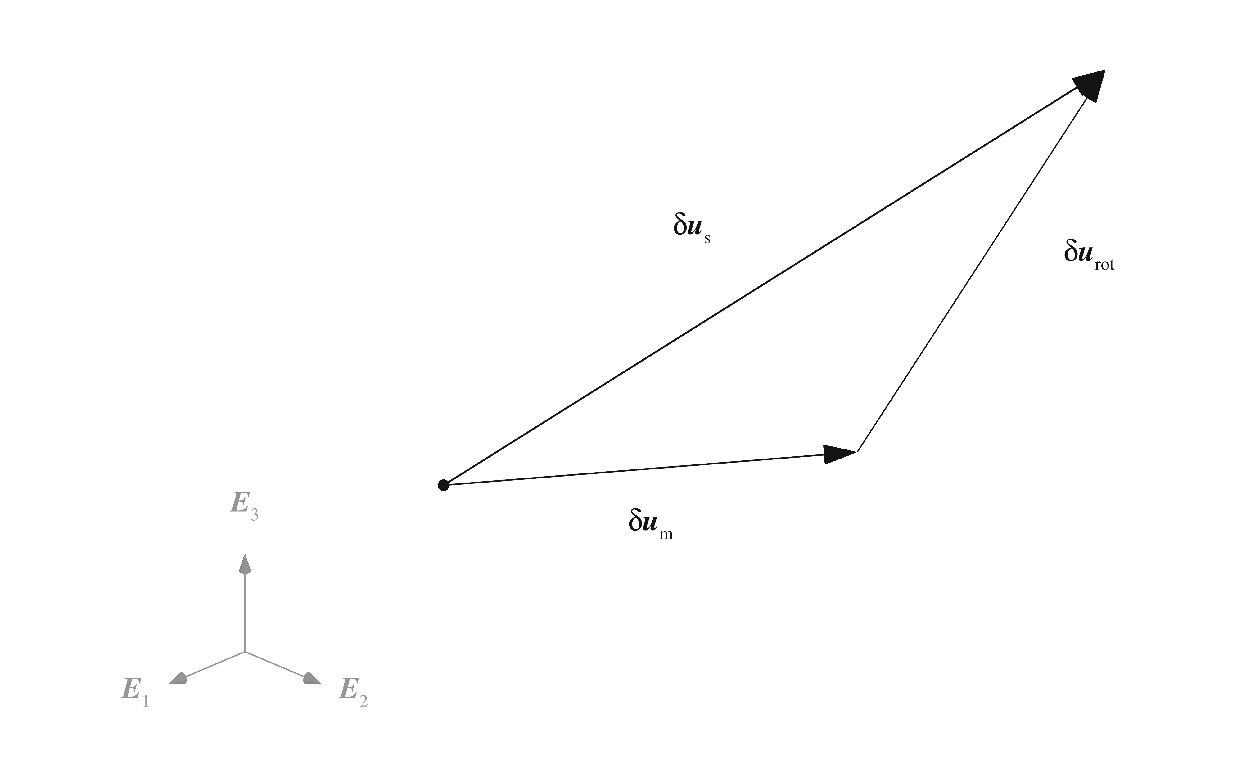
\includegraphics[trim={52.110bp 22.895bp 54.941bp 27.087bp},clip,width=.86\textwidth,height=.31\textheight,keepaspectratio]{figures/tecplot/paper_vinculo_raiz.pdf}
\caption{Incremental compatibility between master $m=H$ and root $s$. Successive arrows represent $\delta\bm u_m$ and $\delta\bm u_{\rm rot}=\delta\bm\theta_m\times\bm r_s$; the direct arrow represents their sum $\delta\bm u_s$. The intermediate point includes only common hub translation.}\label{fig:vinculo-raiz}
\end{figure*}

Derivatives follow by replacing $\bm r_s$ with $\dot{\bm r}_s=\bm W\bm r_s$ and $\ddot{\bm r}_s=\bm W^2\bm r_s$ in the upper-right block; derivatives of the other blocks vanish. Collecting all constraints and support conditions gives $\delta\bm q=\bm T(t)\bm z$, where $\bm z$ contains only independent coordinates. Matrix $\bm T$ retains free columns and inserts blocks $\bm B_s$ in root rows. Equation~\eqref{eq:fullsystem} becomes

\begin{align}
\bm M_r&=\bm T^\tr\bm M\bm T,\nonumber\\
\bm D_r&=\bm T^\tr(\bm D\bm T+2\bm M\dot{\bm T}),\nonumber\\
\bm K_r&=\bm T^\tr(\bm K\bm T+\bm D\dot{\bm T}+\bm M\ddot{\bm T}),\label{eq:dynamicprojection}\\
\bm f_r&=\bm T^\tr\delta\bm f.\nonumber
\end{align}

A static congruence is sufficient only if $\dot{\bm T}=\ddot{\bm T}=\bm0$. Kinematic elimination is neither modal truncation nor a fidelity approximation.

\subsection{Collective and cyclic blade coordinates}
The blade-coordinate transformation, termed \emph{multiblade} in the literature \citep{bir2008}, groups motion into one collective and two cyclic components. It requires equivalent coordinates on the three blades with the same ordering, longitudinal position, and local direction. First construct $\bm H(t)$ with blocks $\operatorname{diag}(\bm Q_b,\bm Q_b)$, where $\bm Q_b=\overline{\bm Q}_{NP_b}$ maps local blade components to inertial components. Roots already constrained to the hub are excluded, and blocks for nonblade coordinates are identities.

For three homologous local values $\zeta_1,\zeta_2,\zeta_3$, write $[\zeta_1,\zeta_2,\zeta_3]^\tr=\bm B_3[y_0,y_c,y_s]^\tr$, with

\begin{equation}
\bm B_3=\begin{bmatrix}
1&\cos\psi_1&\sin\psi_1\\
1&\cos\psi_2&\sin\psi_2\\
1&\cos\psi_3&\sin\psi_3
\end{bmatrix},\qquad
\psi_b=\psi+\frac{2\pi(b-1)}3.
\end{equation}

Coordinate $y_0$ is their mean, and $y_c,y_s$ are the amplitudes of cosine and sine patterns; they are not new physical deformations. If each blade has $n_b$ independent homologous coordinates, use $\bm B_3\otimes\bm I_{n_b}$, where $\otimes$ now denotes the matrix Kronecker product. Adding identities for the remaining coordinates gives $\bm B_{\rm mbc}$. Subscript $\mathrm{mbc}$ identifies only this transformation. Combining it with the basis change gives

\begin{align}
\bm P_{\rm mbc}&=\bm H\bm B_{\rm mbc},\nonumber\\
\dot{\bm P}_{\rm mbc}&=\dot{\bm H}\bm B_{\rm mbc}+\bm H\dot{\bm B}_{\rm mbc},\nonumber\\
\ddot{\bm P}_{\rm mbc}&=\ddot{\bm H}\bm B_{\rm mbc}
+2\dot{\bm H}\dot{\bm B}_{\rm mbc}+\bm H\ddot{\bm B}_{\rm mbc}.
\end{align}

Introducing $\bm z=\bm P_{\rm mbc}\bm y$, matrices $\overline{\bm M},\overline{\bm D},\overline{\bm K}$ follow by applying Eq.~\eqref{eq:dynamicprojection} again, replacing $\bm T$ with $\bm P_{\rm mbc}$ and using input matrices $\bm M_r,\bm D_r,\bm K_r$. Appendix C gives the explicit inverse and derivatives. Gyroscopic effects and derivatives of this coordinate change have different origins and are retained together.

\FloatBarrier
\section{Damping and external actions}
\subsection{Dissipation, gravity, and wind}
Structural damping is represented by the Rayleigh model,

\begin{equation}
\bm C_s=\alpha_R\bm M+\beta_R\bm K_{\rm el},\qquad
\zeta_j=\frac{\alpha_R}{2\omega_j}+\frac{\beta_R\omega_j}{2},
\end{equation}

where $\bm K_{\rm el}$ is global reference elastic stiffness; $\alpha_R$ and $\beta_R$ have units of $\mathrm{s^{-1}}$ and $\mathrm{s}$. Two pairs of angular frequency $\omega_j$ and damping ratio $\zeta_j$ determine the coefficients. This relation applies to modes of the reference conservative system; damping ratios of the operating system follow from its complex eigenvalues. Connection, foundation, and velocity-dependent load contributions are added to $\bm C_s$. The time derivative of mass does not represent dissipation.

Gravitational acceleration is $\bm g=-g\bm E_3$, with $g>0$. Its nodal load uses the same mass distribution. For a two-node element,

\begin{equation}
\bm f_{g,e}=\bm M_e^g[\bm g^\tr,\bm0^\tr,\bm g^\tr,\bm0^\tr]^\tr.
\end{equation}

An eccentric body contributes force $m\bm g$ and moment $\bm r_C\times m\bm g$ at its reference point. In this approximation, gravity loading uses nominal geometry and is independent of the perturbation. If its arm is updated with deformation, its coordinate derivative must also be included in the external-action tangent.

Aerodynamic actions are described by distributed force $\bm p_a$ in $\mathrm{N/m}$ and distributed moment $\bm m_a$ in $\mathrm{N\,m/m}$. Both refer to the section origin and use the same basis as $\bm N$. Conservation of virtual work determines the nodal load:

\begin{equation}
\bm f_{a,e}=\int_0^L\bm N^\tr
\begin{bmatrix}\bm p_a\\\bm m_a\end{bmatrix}\dd x.
\end{equation}

Local relative velocity is $\bm v_{\rm rel}=\bm v_{\rm aire}-\bm v_{\rm estructura}$, evaluated in a common basis and including nominal blade motion. Subscripts $\mathrm{aire}$ and $\mathrm{estructura}$ denote air and structure, respectively. The aerodynamic law relates that velocity and section orientation to $\bm p_a,\bm m_a$. If the resultant acts at a point offset by $\bm r_a$ from the section origin, moment $\bm r_a\times\bm p_a$ is included. The aeroelastic models of \citet{maza2014} provide background for this coupling; choosing the flow law is an assumption additional to the structural formulation. Around the operating state,

\begin{align}
\delta\bm f_a&=\bm F_{a,q}\delta\bm q+\bm F_{a,v}\delta\dot{\bm q}
+\delta\bm f_{a,\rm imp},\nonumber\\
\bm K_a&=-\bm F_{a,q},\qquad \bm C_a=-\bm F_{a,v}.
\end{align}

Matrices $\bm F_{a,q}$ and $\bm F_{a,v}$ are derivatives of nodal loading with respect to coordinates and velocities; $\delta\bm f_{a,\rm imp}$ collects imposed flow variations. A follower load changes direction with structural configuration. Its tangent may be nonsymmetric, so a scalar position potential is not assumed. The same aerodynamic law must be used for equilibrium and these derivatives. Flow with memory additionally requires state variables; instantaneous dependence on position and velocity alone does not represent that memory.

\subsection{Seismic base motion}
Let $\bm\Gamma_f$ transmit uniform ground translation to all nodal coordinates, including supports. For three translational components, it contains identity blocks in translational rows and zeros in angular rows. Acceleration $\bm a_g(t)=\ddot{\bm u}_g(t)$ produces, in independent coordinates before the blade transformation,

\begin{equation}
\bm f_{s,r}(t)=-\bm P_g(t)\bm a_g(t),\qquad
\bm P_g=\bm T^\tr\bm M\bm\Gamma_f.
\label{eq:seismic}
\end{equation}

This form assumes a constant rigid influence and force and dissipation laws defined relative to ground motion. Starting instead from absolute coordinates, substitution of $\delta\bm q_{\rm abs}=\bm T\bm z+\bm\Gamma_f\bm u_g$ generally produces the load

\begin{equation}
-\bm T^\tr(\bm M\bm\Gamma_f\ddot{\bm u}_g
+\bm D\bm\Gamma_f\dot{\bm u}_g+\bm K\bm\Gamma_f\bm u_g).
\end{equation}

The last two terms vanish only if the corresponding matrices annihilate that influence, or if their laws have been defined in relative variables from the outset. An aerodynamic force depending on absolute velocity requires its corresponding contribution to be retained.

The equivalent matrix $\bm\Gamma_{\rm eff}$, defined by $\bm M_r\bm\Gamma_{\rm eff}=\bm P_g$, reproduces base excitation in the reduced equation, but does not replace $\bm\Gamma_f$ when recovering absolute motion. The complete projection retains mass coupling to support coordinates. In collective and cyclic coordinates, loading is additionally multiplied by $\bm P_{\rm mbc}^\tr$.

For a flexible foundation, its coordinates and matrices must remain in the system, and excitation is imposed at the ground interface. Constant stiffness and damping idealize impedance; by themselves, they capture neither soil nonlinearity nor its complete frequency dependence.

\section{Modal and transient problems}
\subsection{Eigenvalues and rigid-body motions}
For the stationary conservative system, the modal problem is

\begin{equation}
\bm K\bm\phi_j=\omega_j^2\bm M\bm\phi_j,\qquad
\bm\phi_i^\tr\bm M\bm\phi_j=\delta_{ij}.
\end{equation}

Vector $\bm\phi_j$ is the vibration mode, $\omega_j$ its angular frequency, and $\delta_{ij}$ the Kronecker delta. The second equality specifies mass normalization. State $\bm q_0$ is not an eigenvector: it is the configuration about which tangent matrices are calculated. For a conservative constant-coefficient system, vibrations can be written as $\delta\bm q(t)=\sum_j\bm\phi_j a_j(t)$, with modal amplitudes $a_j$.
A free twelve-coordinate element admits three infinitesimal translations and three infinitesimal rotations,

\begin{equation}
\bm u_i=\bm a+\bm b\times\bm X_i,\qquad \bm\theta_i=\bm b.
\label{eq:rigid}
\end{equation}

In this expression, $\bm a$ and $\bm b$ are arbitrary infinitesimal translation and rotation; they are not the position vectors used in the \hyperref[sec:giro]{derivation of inertial contributions from prescribed rotation}. Choosing their six unit components successively forms rigid-motion matrix $\bm Q_R$. These motions give $\bm\varepsilon=\bm0$ and $\bm K_e\bm Q_R=\bm0$. For six strictly positive sectional stiffnesses, the deformational complement has positive energy and $\operatorname{rank}(\bm K_e)=6$. With positive-definite mass, the free element has six analytically zero and six positive frequencies. A connected free structure retains six global rigid motions if it has no internal mechanisms; compatible clamping removes them.

The rigid-body nullspace is characterized by zero deformation and elastic energy. It is distinct from prescribed nominal rotation and torsional oscillations of a positive-stiffness connection.

For local operating analysis, matrices in collective and cyclic coordinates are evaluated at a reference azimuth $\psi_\star$. The case $\psi_\star=0$ corresponds to Fig.~\ref{fig:marcos}. Geometry, matrices, and constraints always use the same instant. With $\bm y=\bm\phi e^{\lambda t}$, the quadratic eigenvalue problem follows \citep{tisseur2001}:

\begin{equation}
(\lambda^2\overline{\bm M}+\lambda\overline{\bm D}+\overline{\bm K})\bm\phi=\bm0.
\label{eq:QEP}
\end{equation}

It can be solved without explicitly inverting mass through

\begin{equation}
\begin{bmatrix}\bm0&\I\\-\overline{\bm K}&-\overline{\bm D}\end{bmatrix}
\begin{bmatrix}\bm\phi\\\lambda\bm\phi\end{bmatrix}
=\lambda\begin{bmatrix}\I&\bm0\\\bm0&\overline{\bm M}\end{bmatrix}
\begin{bmatrix}\bm\phi\\\lambda\bm\phi\end{bmatrix}.
\end{equation}

For an oscillatory eigenvalue $\lambda=\sigma+\mathrm i\omega_d$, with $\mathrm i^2=-1$, oscillation frequency is $f_d=|\omega_d|/(2\pi)$. The quantities $f_n=|\lambda|/(2\pi)$ and $\zeta=-\sigma/|\lambda|$ may also be defined as parameters of the complex pair. The sign of $\sigma$ indicates growth or decay in the local constant-coefficient system. If matrices retain periodic time dependence, this local problem alone does not determine periodic-motion stability.

\subsection{Reduced-order projection}
A constant basis $\bm V$ introduces $\bm y\simeq\bm V\bm\xi$ and gives

\begin{equation}
\bm M_{\rm red}=\bm V^\tr\overline{\bm M}\bm V,\quad
\bm D_{\rm red}=\bm V^\tr\overline{\bm D}\bm V,\quad
\bm K_{\rm red}=\bm V^\tr\overline{\bm K}\bm V.
\end{equation}

Matrix $\bm V$ contains the chosen basis vectors, and $\bm\xi$ their amplitudes; loading is projected with $\bm V^\tr$. For the conservative case, a mass-orthonormal modal basis may be chosen. With rotation, selection must retain couplings relevant to the state considered. A time-dependent basis introduces its own derivatives according to Eq.~\eqref{eq:dynamicprojection}. This lower-dimensional approximation is distinct from exact elimination of dependent coordinates through $\bm T$.

\subsection{Integration and physical recovery}
Time integration can be performed in independent coordinates $\bm z$, before the blade transformation. Local analysis keeps $\bm M_r,\bm D_r,\bm K_r$ constant, evaluated at the same operating state. For time $t_n$ and step $\Delta t=t_{n+1}-t_n$, Newmark's average-acceleration method is defined by

\begin{align}
\bm z_{n+1}&=\bm z_n+\Delta t\dot{\bm z}_n
+\tfrac{\Delta t^2}{4}(\ddot{\bm z}_n+\ddot{\bm z}_{n+1}),\nonumber\\
\dot{\bm z}_{n+1}&=\dot{\bm z}_n+\tfrac{\Delta t}{2}
(\ddot{\bm z}_n+\ddot{\bm z}_{n+1}).
\end{align}

The effective matrix is $\bm K_r+4\bm M_r/\Delta t^2+2\bm D_r/\Delta t$; it is retained in full even when nonsymmetric. Appendix C gives the right-hand side. Numerical integration stability and physical system stability are different properties.

For $\delta\bm q=\bm T(t)\bm z$, recovery requires

\begin{align}
\delta\dot{\bm q}&=\bm T\dot{\bm z}+\dot{\bm T}\bm z,\nonumber\\
\delta\ddot{\bm q}&=\bm T\ddot{\bm z}+2\dot{\bm T}\dot{\bm z}+\ddot{\bm T}\bm z.
\end{align}

Term $\bm\Gamma_f\bm a_g$ is added to recover absolute perturbation acceleration; nominal centripetal acceleration is included separately when total acceleration is required. When matrices are evaluated at fixed azimuth, $\bm T,\dot{\bm T},\ddot{\bm T}$ are also evaluated there: reconstruction is local and does not describe a complete periodic trajectory.

Reactions are recovered from the complete residual of Eq.~\eqref{eq:fullsystem}, before eliminating supports and constraints. Their projection onto admissible coordinates vanishes. The six-component incremental resultants are $[\delta\bm n^\tr,\delta\bm m_s^\tr]^\tr=\bm K_s\bm B\bm T_e\delta\bm q_e^g$. Total resultants additionally include those of equilibrium $\bm q_0$.

\section{Conclusions}
The formulation relates the material description of components to nominal motion, sectional properties, and discrete perturbation equations. Defined reference frames and a consistent transformation convention distinguish rotor rotation from deformation of the tower, nacelle, hub, and blades.

The gyroscopic matrix follows from the skew-symmetric part of velocity--displacement coupling in kinetic energy. Transport to fixed axes and time-dependent constraints introduce additional contributions that must be retained together. Equilibrium and linearization place inertial terms on the left-hand side and external actions on the right.

The model assumes small structural deformations, reference mass properties, and constant nominal angular velocity. These assumptions support local vibration and transient-response analysis about an operating state. Periodic excitations or coefficients must remain in the time-dependent problem; a fixed-azimuth evaluation does not solve that regime. The formulation establishes the relations needed to incorporate aerodynamic and foundation laws consistent with these assumptions.

\section{Appendix A. Element matrices and interpolation}
Element ordering is $\bm q_e^\ell=[(\bm q_I^\ell)^\tr,(\bm q_J^\ell)^\tr]^\tr$, where $\bm q_i^\ell=[u_i,v_i,w_i,\theta_{xi},\theta_{yi},\theta_{zi}]^\tr$. Extension, at indices $(1,7)$, and torsion, at $(4,10)$, use

\begin{equation}
\bm K_{\rm ax}=\frac{EA}{L}\begin{bmatrix}1&-1\\-1&1\end{bmatrix},\qquad
\bm K_{\rm tor}=\frac{GJ_t}{L}\begin{bmatrix}1&-1\\-1&1\end{bmatrix}.
\end{equation}

For each plane, define

\begin{align}
\phi&=\frac{12EI}{GA_sL^2},&a&=\frac{12EI}{L^3(1+\phi)},\nonumber\\
b&=\frac{6EI}{L^2(1+\phi)},&c&=\frac{(4+\phi)EI}{L(1+\phi)},\nonumber\\
d&=\frac{(2-\phi)EI}{L(1+\phi)}.
\end{align}

The bending block is

\begin{equation}
\bm K_{\rm fl}=\begin{bmatrix}
a&rb&-a&rb\\rb&c&-rb&d\\-a&-rb&a&-rb\\rb&d&-rb&c
\end{bmatrix}.
\end{equation}

Use $(EI_z,GA_{sy},r=1)$ at indices $(2,6,8,12)$ and $(EI_y,GA_{sz},r=-1)$ at $(3,5,9,11)$. Inserting the four blocks determines all entries of $\bm K_e^\ell$.

For $s=x/L$ and $\bm p=[1,s,s^2,s^3]$, interpolation in one plane is $v=\bm p\bm C_v\bm d_y$, $\theta_z=\bm p\bm C_r\bm d_y$, with $\bm d_y=[v_I,\theta_{zI},v_J,\theta_{zJ}]^\tr$ and

\begin{equation}
\bm C_v=\frac1{1+\phi}\begin{bmatrix}
1+\phi&0&0&0\\
-\phi&L(1+\phi/2)&\phi&-L\phi/2\\
-3&-L(2+\phi/2)&3&-L(1-\phi/2)\\
2&L&-2&L
\end{bmatrix},
\end{equation}

\begin{equation}
\bm C_r=\frac1{1+\phi}\begin{bmatrix}
0&1+\phi&0&0\\
-6/L&-(4+\phi)&6/L&-(2-\phi)\\
6/L&3&-6/L&3\\0&0&0&0
\end{bmatrix}.
\end{equation}

For the other plane, use $\bm d_z=[w_I,\theta_{yI},w_J,\theta_{yJ}]^\tr$, $\bm S_z=\operatorname{diag}(1,-1,1,-1)$, $w=\bm p\bm C_v\bm S_z\bm d_z$, and $\theta_y=-\bm p\bm C_r\bm S_z\bm d_z$, with the corresponding $\phi$. Fields $u,\theta_x$ are interpolated linearly. These relations define $\bm N$; their derivatives and shear terms define $\bm B$.

For constant properties, four Gauss points exactly integrate mass and gyroscopic products of maximum degree six. The preceding stiffness is available in closed form, rather than through reduced integration. Coupled-section formulations require constructing and discretizing their general energy; arbitrary coupling entries cannot simply be inserted into these four blocks.

\section{Appendix B. Energy derivatives}
The relation between $\dot{\bm\theta}$ and angular velocity is given by~\eqref{eq:jacobiano}. To verify the gyroscopic contribution, differentiate the velocity terms of~\eqref{eq:T2} with constant coefficients:

\begin{align}
\frac{\dd}{\dd t}\frac{\partial\mathcal T_v^{(2)}}{\partial\dot{\bm\eta}}
&=\bm M_6\ddot{\bm\eta}+\bm A_6\dot{\bm\eta},\nonumber\\
\frac{\partial\mathcal T_v^{(2)}}{\partial\bm\eta}
&=\bm A_6^\tr\dot{\bm\eta}.
\end{align}

Subtracting gives $\bm M_6\ddot{\bm\eta}+\bm G_{c,6}\dot{\bm\eta}$, with $\bm G_{c,6}=\bm A_6-\bm A_6^\tr$. The remaining inertial term follows by applying~\eqref{eq:inercia-generalizada} to the complete energy and corresponds to~\eqref{eq:tangente-inercial}. Explicitly time-dependent coefficients would additionally produce $\dot{\bm M}_6\dot{\bm\eta}$ and $\dot{\bm A}_6\bm\eta$.

For external torque $\bm\tau$ in nominal components, virtual work is $\delta W=\bm\tau^\tr\bm J_\ell\delta\bm\theta$ and its generalized action is $\bm Q_\tau=\bm J_\ell^\tr\bm\tau$. If $\bm\tau=\bm\tau_0$ remains constant in that basis, linearization gives $\bm Q_\tau=\bm\tau_0+\tfrac12\Sx{\tau_0}\bm\theta$. If it remains constant in the body, $\bm\tau=\bm E\bm\tau_0$ and $\bm Q_\tau=\bm\tau_0-\tfrac12\Sx{\tau_0}\bm\theta$. The matrix entering the left-hand side is $-\partial\bm Q_\tau/\partial\bm\theta$. This example distinguishes physical torque from the generalized components conjugate to the rotation vector.

The corotational energy in Eq.~\eqref{eq:corot} allows internal force and tangent evaluation through central differences. For coordinate increments $h_i$,

\begin{align}
f_i&\simeq\frac{U(\bm q+h_i\bm e_i)-U(\bm q-h_i\bm e_i)}{2h_i},\nonumber\\
K_{ii}&\simeq\frac{U(\bm q+h_i\bm e_i)-2U(\bm q)+U(\bm q-h_i\bm e_i)}{h_i^2},\nonumber\\
K_{ij}&\simeq\frac{U_{++}-U_{+-}-U_{-+}+U_{--}}{4h_ih_j},\quad i\ne j,
\end{align}

where $U_{\pm\pm}=U(\bm q\pm h_i\bm e_i\pm h_j\bm e_j)$. Steps must respect coordinate scales and dimensions. This procedure approximates derivatives of one energy; it does not turn approximate kinematics into a geometrically exact beam.

A linear initial-stress alternative uses

\begin{equation}
U_g=\frac{N_0}2\int_0^L[(v')^2+(w')^2]\dd x,
\qquad \bm K_g=N_0\int_0^L\bm N_\perp'{}^\tr\bm N_\perp'\dd x,
\end{equation}

with $N_0>0$ in tension. For one plane and the interpolation in Appendix A,

\begin{equation}
\bm K_g^{(p)}=\frac{N_0}{(1+\phi)^2}\begin{bmatrix}
a_g/L&r/10&-a_g/L&r/10\\
r/10&Lc_g&-r/10&-Ld_g\\
-a_g/L&-r/10&a_g/L&-r/10\\
r/10&-Ld_g&-r/10&Lc_g
\end{bmatrix},
\end{equation}

where $a_g=\phi^2+2\phi+6/5$, $c_g=\phi^2/12+\phi/6+2/15$, and $d_g=\phi^2/12+\phi/6+1/30$. This expression explains the axial-force contribution; it is not added to a Hessian already containing the same preload.

\section{Appendix C. Transformations and time integration}
The mass derivative after constraints is

\begin{align}
\dot{\bm M}_r={}&\dot{\bm T}^\tr\bm M\bm T+\bm T^\tr\dot{\bm M}\bm T
+\bm T^\tr\bm M\dot{\bm T}.
\end{align}

This identity again separates the mass derivative from the skew-symmetric part of the inertial velocity matrix.

The inverse collective--cosine--sine transformation and derivatives of the forward transformation are

\begin{equation}
\bm B_3^{-1}=\frac13\begin{bmatrix}
1&1&1\\2\cos\psi_1&2\cos\psi_2&2\cos\psi_3\\
2\sin\psi_1&2\sin\psi_2&2\sin\psi_3
\end{bmatrix},
\end{equation}

\begin{align}
[\dot{\bm B}_3]_{b,:}&=\Omega[0,-\sin\psi_b,\cos\psi_b],\nonumber\\
[\ddot{\bm B}_3]_{b,:}&=-\Omega^2[0,\cos\psi_b,\sin\psi_b].
\end{align}

For blade blocks, $\dot{\bm H}=\bm W_H\bm H$ and $\ddot{\bm H}=\bm W_H^2\bm H$. Matrix $\bm W_H$ repeats $\bm W$ in blade translational and angular blocks and is zero elsewhere. These derivatives do not vanish when an evaluation azimuth is selected.

To complete the average-acceleration time step, define

\begin{align}
\bm K_{\rm eff}&=\bm K_r+\frac4{\Delta t^2}\bm M_r+\frac2{\Delta t}\bm D_r,\nonumber\\
\bm f_{\rm eff}&=\bm f_{n+1}
+\bm M_r\left(\frac4{\Delta t^2}\bm z_n+\frac4{\Delta t}\dot{\bm z}_n+\ddot{\bm z}_n\right)\nonumber\\
&\quad+\bm D_r\left(\frac2{\Delta t}\bm z_n+\dot{\bm z}_n\right),\nonumber\\
\bm K_{\rm eff}\bm z_{n+1}&=\bm f_{\rm eff}.
\end{align}

Here, $\bm f_{n+1}=\bm f_r(t_{n+1})$ is the projected load at the new time. Velocities and accelerations follow from the Newmark relations. The same scheme applies to a reduced-order system, with loads and initial conditions projected as well \citep{newmark1971}.

\section{Declaration on the use of artificial intelligence}
ChatGPT (OpenAI) was used to assist in organizing and drafting the manuscript, translating it, and reviewing the correspondence between mathematical expressions and project code. The tool also assisted in developing and reviewing the computational implementation of the formulation. The authors are responsible for the accuracy, originality, and interpretation of the content.
